\documentclass[12pt,oneside]{uhthesis}
\usepackage{subfigure}
\usepackage[ruled,lined,linesnumbered,titlenumbered,algochapter,spanish,onelanguage]{algorithm2e}
\usepackage{amsmath}
\usepackage{amssymb}
\usepackage{amsbsy}
\usepackage{caption,booktabs}
\captionsetup{ justification = centering }
%\usepackage{mathpazo}
\usepackage{float}
\setlength{\marginparwidth}{2cm}
\usepackage{todonotes}
\usepackage{listings}
\usepackage{xcolor}
\usepackage{multicol}
\usepackage{graphicx}
\floatstyle{plaintop}
\restylefloat{table}
\addbibresource{Bibliography.bib}
% \setlength{\parskip}{\baselineskip}%
\renewcommand{\tablename}{Tabla}
\renewcommand{\listalgorithmcfname}{Índice de Algoritmos}
%\dontprintsemicolon
\SetAlgoNoEnd

\definecolor{codegreen}{rgb}{0,0.6,0}
\definecolor{codegray}{rgb}{0.5,0.5,0.5}
\definecolor{codepurple}{rgb}{0.58,0,0.82}
\definecolor{backcolour}{rgb}{0.95,0.95,0.92}

\lstdefinestyle{mystyle}{
    backgroundcolor=\color{backcolour},   
    commentstyle=\color{codegreen},
    keywordstyle=\color{purple},
    numberstyle=\tiny\color{codegray},
    stringstyle=\color{codepurple},
    basicstyle=\ttfamily\footnotesize,
    breakatwhitespace=false,         
    breaklines=true,                 
    captionpos=b,                    
    keepspaces=true,                 
    numbers=left,                    
    numbersep=5pt,                  
    showspaces=false,                
    showstringspaces=false,
    showtabs=false,                  
    tabsize=4
}

\lstset{style=mystyle}

\title{Título de la tesis}
\author{\\\vspace{0.25cm}Alex Sierra Alcalá}
\advisor{\\\vspace{0.25cm}Nombre del primer tutor\\\vspace{0.2cm}Nombre del segundo tutor}
\degree{Licenciado en (Matemática o Ciencia de la Computación)}
\faculty{Facultad de Matemática y Computación}
\date{Fecha\\\vspace{0.25cm}\href{https://github.com/username/repo}{github.com/username/repo}}
\logo{Graphics/uhlogo}
\makenomenclature

\renewcommand{\vec}[1]{\boldsymbol{#1}}
\newcommand{\diff}[1]{\ensuremath{\mathrm{d}#1}}
\newcommand{\me}[1]{\mathrm{e}^{#1}}
\newcommand{\pf}{\mathfrak{p}}
\newcommand{\qf}{\mathfrak{q}}
%\newcommand{\kf}{\mathfrak{k}}
\newcommand{\kt}{\mathtt{k}}
\newcommand{\mf}{\mathfrak{m}}
\newcommand{\hf}{\mathfrak{h}}
\newcommand{\fac}{\mathrm{fac}}
\newcommand{\maxx}[1]{\max\left\{ #1 \right\} }
\newcommand{\minn}[1]{\min\left\{ #1 \right\} }
\newcommand{\lldpcf}{1.25}
\newcommand{\nnorm}[1]{\left\lvert #1 \right\rvert }
\renewcommand{\lstlistingname}{Ejemplo de código}
\renewcommand{\lstlistlistingname}{Ejemplos de código}

\begin{document}

\frontmatter
\maketitle

\begin{dedication}
    A mi familia, en especial a mis padres.
\end{dedication}
\begin{acknowledgements}
    Agradecimientos
\end{acknowledgements}
\begin{opinion}
    Opiniones de los tutores
\end{opinion}
\begin{resumen}
	Resumen en español
\end{resumen}

\begin{abstract}
	Resumen en inglés
\end{abstract}
\tableofcontents
\listoffigures
% \listoftables
% \listofalgorithms
\lstlistoflistings

\mainmatter

\chapter*{Introducción}\label{chapter:introduction}
\addcontentsline{toc}{chapter}{Introducción}

En la era del big data, la capacidad de analizar e interpretar datos complejos de trayectorias humanas se ha convertido en un elemento esencial para comprender y gestionar dinámicas sociales, urbanas y ambientales. Este análisis, impulsado por datos recolectados a través de la telefonía móvil, no solo permite identificar patrones de movilidad humana, sino que también informa la planificación urbana, optimiza el transporte y guía la formulación de políticas públicas. Sin embargo, estos datos suelen ser incompletos o dispersos debido a factores como la pérdida de señal o limitaciones en las capacidades de seguimiento, lo que hace imprescindible desarrollar estrategias eficaces para su completamiento.

En contextos de desarrollo como Cuba, donde la digitalización está en crecimiento, pero los recursos y datos disponibles son limitados, los datos recolectados mediante la telefonía móvil ofrecen una oportunidad invaluable. No obstante, la dispersión, incompletitud e irregularidad en el tiempo de los datos, debido a apagones y averías en el sistema de telecomunicaciones, dificultan en gran medida este proceso. Dentro de este panorama, el completamiento de trayectorias humanas a partir de datos escasos representa un reto significativo en nuestro país, de ahí la necesidad de desarrollar soluciones adaptadas a nuestras particularidades.

\section*{Datos de telefonía móvil}

El crecimiento sostenido de la población humana, junto con su concentración en áreas urbanas y el aumento de su movilidad, ha planteado retos significativos para la adaptación de los sistemas sociales y demográficos. Estas dinámicas impactan directamente en la planificación y desarrollo de políticas públicas, ya que entender los patrones de movilidad resulta crucial para abordar problemas en diversas áreas. Por ejemplo, en la planificación del transporte, conocer cómo se desplazan las personas permite diseñar redes de carreteras más eficientes y sistemas de transporte público mejor adaptados a las necesidades de la población. En el ámbito de la salud, el modelado de la propagación de enfermedades infecciosas se beneficia de estos datos, ya que facilita la implementación de restricciones y controles más efectivos. Además, en el sector comercial, el geomarketing utiliza los patrones de movilidad para optimizar la distribución geográfica de publicidad y anuncios, maximizando su impacto \cite{asgari2013survey}.

Históricamente, el análisis de la movilidad humana se basaba en métodos tradicionales como encuestas, observación directa o censos poblacionales. Aunque útiles, estos enfoques presentan limitaciones significativas debido a su elevado costo, frecuencia limitada y dependencia de muestras pequeñas, lo que dificulta obtener una visión integral de los flujos de movilidad \cite{asgari2013survey}. En las últimas décadas, el desarrollo tecnológico ha permitido explorar nuevas fuentes de datos. Algunos estudios como \cite{gong2012gps} hacen uso de los sistemas GPS, que ofrecen una alta precisión en exteriores, sin embargo su uso puede ser intermitente debido al consumo de batería de los dispositivos, y por lo general requieren de la instalación de software específico y la activación del mismo por parte del usuario. Esto implica que los estudios basados en GPS suelan estar limitados a pequeñas muestras. Una alternativa, menos precisa pero mucho más abarcadora, es el uso de datos provenientes de las redes de telecomunicaciones, en particular los registros generados por los teléfonos móviles. Estos dispositivos, que actualmente son utilizados por el 80$\%$ de la población mundial mayor de 10 años y hasta el 90$\%$ en regiones como América y Europa \cite{ITU2024}, recopilan una cantidad masiva de datos vinculados a la actividad de sus usuarios \cite{toole2015path} que se requieren para el correcto funcionamiento de la red.

Los registros de telefonía móvil incluyen información como la identificación anónima del usuario, la ubicación de las radio bases con las que interactúan sus dispositivos y marcas temporales, permitiendo rastrear trayectorias de movilidad en tiempo real. Esto convierte a los teléfonos móviles en una plataforma de censado masivo de la actividad humana \cite{doyle2014population}, que no solo es económica y escalable, sino también capaz de proporcionar una visión general de los desplazamientos individuales y colectivos. Estas trayectorias ofrecen información valiosa para el análisis de la movilidad humana, contribuyendo a la toma de decisiones en múltiples campos y representando un recurso crucial para la investigación y el desarrollo de soluciones basadas en datos.

\subsection*{Registros de Telefonía Móvil}

Una red de telefonía celular se compone de una infraestructura de radio desplegada en áreas denominadas celdas, cada una equipada con al menos una estación base transmisora-receptora fija (BTS, por sus siglas en inglés, \textit{base transceiver station}) \cite{sharma2012cell}. Estas estaciones permiten establecer conexiones inalámbricas entre los terminales de los usuarios y la red en cualquier momento. Las interacciones generadas entre los dispositivos móviles y las BTS se almacenan en registros que contienen información clave, como identificadores de los usuarios y de las estaciones a las que se conectan \cite{yuan2013characterizing}. La estructura y el tipo de registros generados pueden variar según la tecnología utilizada por el proveedor de la red, aunque ciertos estándares han sido adoptados de manera general \cite{durive2021sistema}.

Entre los registros de mayor interés para estudios de movilidad se encuentran los Call Detail Records (CDR) y los Location Update Records (LUR) \cite{gutierrez2020como}. Los CDR se generan durante eventos específicos, como llamadas, mensajes o conexiones a la red, y son comúnmente utilizados para la facturación de los usuarios, lo que asegura su almacenamiento por largos períodos. Estos registros incluyen información como identificadores de los dispositivos, marcas de tiempo y tipos de eventos, siendo ampliamente utilizados en estudios de movilidad gracias a su disponibilidad. Por otro lado, los LUR son activados por la red en situaciones como cambios de cobertura o períodos de inactividad, proporcionando una mayor resolución temporal al registrar eventos independientes de las actividades de los usuarios. Sin embargo, debido a que no son utilizados para facturación, suelen ser desechados, lo que limita su aplicación en estudios de movilidad \cite{durive2021sistema}.

A pesar de las diferencias en los eventos que generan estos registros, ambos comparten una estructura de información similar, incluyendo identificadores, eventos, celdas y marcas temporales. Estos datos permiten aproximar las localizaciones de los usuarios en diferentes momentos, aunque la resolución espacial depende de la densidad de las BTS, la cual varía significativamente entre áreas urbanas y rurales \cite{forghani2020cellular}. Al identificar registros con el mismo identificador de usuario, es posible reconstruir trayectorias aproximadas que muestran las posiciones de las estaciones base a las que un dispositivo se conectó mientras se desplazaba \cite{chen2018individual}. En este contexto, una colección de trayectorias derivadas de datos de telefonía móvil puede ofrecer una representación aproximada de la movilidad.

\subsection*{Desafíos}

Los datos de redes de telecomunicaciones han revolucionado los estudios de movilidad humana al proporcionar grandes volúmenes de información que superan las limitaciones de métodos tradicionales como las encuestas. Aunque estos datos han abierto nuevas posibilidades para investigar patrones de movilidad, también presentan desafíos significativos.

Uno de los principales retos es garantizar la privacidad de los usuarios, la cual ha recibido mucha atención en los años recientes. La protección de información sensible ha llevado a restricciones en el acceso a los registros, incluso cuando están anonimizados. Por ejemplo en \cite{tesselkin2017estimation} se presenta un modelo de red de transporte en forma de cadena de Markov para la estimación de las matrices origen-destino (O-D). Con cierta similitud, en \cite{pourmoradnasseri2019od} un modelo de Markov de segundo orden es empleado bajo la premisa de investigar patrones de movilidad humanos a partir de telefonía celular. Resultando de interés, en particular, la determinación de matrices O-D y el completamiento de trayectoria.

A pesar de los avances, el balance entre el aprovechamiento de los datos y la protección de la privacidad sigue siendo una barrera crítica en la investigación, especialmente en contextos donde el acceso a datos es fundamental para obtener resultados significativos.

% % \subsection*{Antecedentes}

% % Este último apartado, el de el completamiento de trayectorias, ha recibido especial atención debido a las limitaciones relacionadas con la resolución temporal y espacial de los registros de telefonía móvil. Se ha presentado un amplio grupo de metodologías orientadas hacia este problema, frecuentemente uniendo datos de telefonía con la estructura de alguna red de transporte. Contando estas metodologías con un grupo de limitaciones.

% % Se pueden encontrar algunas metodologías de completamiento basadas en interpolación, como el caso de [20]. La interpolación, en general, es precisa cuando la densidad de puntos es elevada, lo cual no suele ser el caso de los registros de telefonía, ademas de que no suele usar información de trayectorias similares para el completamiento. De forma similar [21] realiza el completamiento uniendo nodos para lograr el camino mas corto dentro de una red de transito a la cual son mapeadas las localizaciones de los registros y Vajakas et al. [22] propone un completamiento basado en asignar el camino mas rápido entre los dos puntos de la red de transito de la cual se tengan registros consecutivos.

% % Por su parte, [23] utiliza la periodicidad en la movilidad humana y la factorización de tensores para completar trayectorias individuales, para lo cual se necesitan datos de un mismo usuario por un largo periodo de tiempo. Otros trabajos orientados al completamiento de trayectorias complementan los registros con información topológica [15] o información sobre el \textit{handoff} entre torres [24].

% % El marco GRFTrajRec aborda los desafíos de datos de trayectorias urbanas de baja frecuencia mediante una innovadora representación basada en grafos que integra dimensiones de red y trayectoria. Con un modelo seq2seq sensible a intervalos espaciotemporales, GRFTrajRec captura atributos esenciales en los puntos de trayectoria, permitiendo restaurar puntos GPS ausentes con alta precisión.

% % Una buena parte de los trabajos orientados al completamiento de trayectorias de movilidad utilizan técnicas de \textit{machine learning} o redes neuronales artificiales (ANN, por \textit{artifcial neural network}). Por ejemplo, en [25] se presenta una métodología para reconstruir trayectorias a partir de imágenes, utilizando una ANN para refnar las trayectorias después de una etapa de \textit{clustering}. Zhang et al. [26] propone una red neuronal profunda combinando redes convolucionales, secuenciales y dos mecanismos de atención para estimar localizaciones en exteriores a partir de información de la red de telefonía que incluye datos de la intensidad de la señal del usuario respecto a diferentes torres. La trayectoria se reconstruye a partir de las localizaciones estimadas a partir de una técnica de \textit{map-matching} presentada en [27].

\subsection*{Historia en Cuba}

La Empresa de Telecomunicaciones de Cuba, Etecsa, es la única empresa en el territorio nacional que provee servicios de telefonía móvil e Internet. A pesar de grandes avances los últimos años, estos servicios demoraron más tiempo para hacerse populares y accesibles a la mayor parte de la población cubana respecto a la media mundial \cite{durive2021sistema}. Como consecuencia directa, la experiencia con el uso de datos de la red de telefonía celular para estudios de movilidad en Cuba esta limitada a años recientes.

Según se relata en \cite{durive2021sistema}, en 2018 comienza un esfuerzo por parte de investigadores del actual Centro de Sistemas Complejos de la Facultad de Física de la Universidad de La Habana para acceder a los registros de telefonía celular con el objetivo de extraer analítica que enriqueciera los procesos de toma de decisiones por parte de las autoridades de salud, planificación del transporte y estudios socio-demográficos, etc. Obteniéndose el acceso a registros de tipo LUR a partir del año 2020, acordándose con Etecsa la firma de un acuerdo de confidencialidad con la universidad y el compromiso de respetar una serie de métodos de seguridad entre los que figura que:

\begin{itemize}
    \item los datos de LUR son almacenados en servidores de Etecsa, dentro de la red de la compañía;
    \item los datos son almacenados sin identificadores de usuarios, como nombre, teléfono o IMSI;
    \item ningún dato de granularidad individual puede sustraerse de la red de la empresa;
    \item ningún procedimiento de ingeniera inversa o \textit{de-anonymization} puede usarse;
    \item los datos se entregan con fines de investigación y solo pueden usarse para estos fines;
    \item Etecsa emite por escrito autorización para la divulgación de los resultados obtenidos.
\end{itemize}

Etecsa ha desplegado más de 1,500 radiobases en Cuba, con una distribución heterogénea que refleja la densidad de usuarios, concentrándose en áreas urbanas. Para proteger la ubicación precisa de estas torres, se adoptó una estrategia que agrupa torres cercanas en zonas densas y ajusta ligeramente su posición en zonas rurales, reduciendo el número a 795 pseudo-torres con ubicaciones GPS compartidas. Estas pseudo-torres se emplean en estudios de movilidad mediante zonas de cobertura definidas con celdas de Voronoi, funcionando de manera similar a las torres reales para los análisis realizados.

El estudio de la movilidad poblacional a partir de los registros LUR de la empresa Etecsa está amparado por la legislación cubana. En particular la Ley de protección de Datos Personales \cite{cuervo2022resolucion}, del 2022, define lo que se consideran datos personales (que incluye los datos generados por sistemas tecnológicos como los teléfonos) y las reglas para su uso. Estipula que dichos datos pueden usarse por razones de bienestar general si se someten previamente a un procedimiento de disociación, como el antes mencionado.

El valor social de comprender y usar estos datos quedó demostrado ampliamente cuando en medio de la pandemia de SARS-CoV2 a partir de marzo de 2020, el sistema de salud y el gobierno cubanos pudieron disponer de modelos de movilidad para evaluar la efectividad de las medidas de limitación de movimiento que se implementaron. Es importante resaltar que, durante ese mismo período, la mayor parte de los gobiernos del mundo usaron métricas semejantes para entender la epidemia y sus consecuencias. En muchos casos, los modelos de movilidad provinieron de empresas como Google, que amparada por la urgencia médica mundial, puso a disposición de los investigadores modelos de movilidad basados en la detección de posicionamiento de los usuarios a partir de los metadatos generados por sus aplicaciones. Es de señalar que Google excluyó a Cuba de la lista de países que podían acceder a dichos datos, como se muestra en la figura \ref{fig:google_exclusion}.

\begin{figure}[!htb] \centering 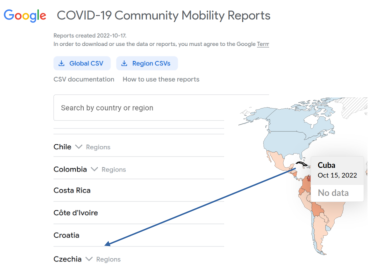
\includegraphics[width=0.5\textwidth]{Graphics/google_exclusion.pdf} \caption{Cuba excluida por Google en el acceso a datos de movilidad} \label{fig:google_exclusion} \end{figure}

Si bien los modelos de movilidad generados por el Centro de Sistemas Complejos, de acuerdo con Etecsa, fueron de gran utilidad, es importante señalar que dichos datos tienen menos precisión y menos abundantes que los que disponen empresas como Google, Facebook y otras.

Una de las enseñanzas de la pandemia y de la posterior aplicación de estos datos al estudio de la movilidad poblacional es que no se puede esperar a tener situaciones críticas para decidirse a usar estos métodos de Big Data. Esencialmente, aunque el posible uso y valor de estos datos sea bastante obvio, en los detalles de cómo extraer valor informacional radica un gran reto. Es importante crear una base científica y tecnológica que permita, ante necesidades concretas, saber las potencialidades de estos datos, si permiten o no enfrentar la tarea en cuestión, y la precisión de los mismos.

% % En los últimos años, diversas investigaciones han explorado métodos para el completamiento y la predicción de trayectorias, abarcando desde técnicas clásicas de interpolación hasta enfoques más recientes de aprendizaje profundo. La competencia HuMob (Human Mobility) Challenge ha tenido un gran impacto en este campo, ya que se propone anualmente romper el estado del arte de los modelos computacionales para la predicción de patrones de movilidad humana. Lamentablemente, la mayoría de los estudios están casi siempre orientados a entornos con abundancia de datos, dejando una brecha en la literatura sobre contextos con datos limitados. Destacan entonces enfoques como el de GRFTrajRec con una representación de trayectorias basada en grafos, la cual mejora la comprensión de las interacciones entre trayectorias y redes viales. Este sistema, usando un modelo seq2seq basado en intervalos espaciotemporales, ha demostrado aumentar la precisión y la consistencia espacial en las predicciones utilizando datos reales. Otra investigación basada en factorización tensorial, en conjunto con datos de registros de llamadas o CDR (por sus siglas en ingles, \textit{call detail records}), permite reconstruir trayectorias individuales con alta precisión, incluso con solo el 1$\%$ de los datos originales.

% % El uso de datos de telefonía en Cuba ha permitido analizar patrones de movilidad en diversas situaciones, como durante la pandemia de COVID-19, y ha sido fundamental en la integración de modelos para la propagación de epidemias. De igual forma, estudios han aprovechado estos datos para actualizar áreas de ubicación y comprender los flujos de movilidad entre zonas de transporte, lo que contribuye significativamente a la toma de decisiones y al control de crisis.

\section*{Objetivos y estructura del documento}

Teniendo en cuenta los datos disponibles en el Centro de Sistemas Complejos y las condiciones pactadas con la empresa de telecomunicaciones para el uso de los mismos, esta investigación se plantea atender el problema de completar trayectorias de movilidad humana a partir de registros de telefonía móvil, utilizando métodos que consideren la baja densidad de los datos. El objetivo fundamental es el de contribuir a la creación de modelos de movilidad más preciso a partir del completamiento de datos que suelen ser imprecisos e incompletos.

A diferencia de investigaciones cubanas anteriores, este trabajo se centra en evaluar la aplicabilidad y el desempeño de TrajBERT \cite{si2023trajbert}, un modelo basado en la arquitectura de \textit{transformer} \cite{vaswani2017attention} que permite aprovechar la información espaciotemporal. Este estudio se enfoca en adaptar el modelo a las particularidades locales, al emplear datos cubanos recolectados mediante telefonía móvil. Finalmente, se busca identificar tanto las fortalezas como las limitaciones del modelo, contribuyendo al avance del conocimiento en el campo.

Por tanto el objetivo general que rige este estudio es investigar la aplicabilidad y adaptabilidad del modelo TrajBERT para el completamiento de trayectorias humanas en el contexto cubano, utilizando datos recolectados mediante telefonía móvil.

Para cumplir el objetivo general se definen los siguientes objetivos específicos:

\begin{enumerate}
    \item Investigar la literatura relacionada con el tema y con las herramientas tecnológicas utilizadas, como el aprendizaje profundo y las arquitecturas basadas en \textit{transformer}.
    \item Analizar las fortalezas y debilidades del modelo TrajBERT en el contexto del completamiento de trayectorias, mediante la evaluación de su arquitectura y capacidades técnicas.
    \item Implementar TrajBERT utilizando una base de datos de trayectorias cubanas para evaluar su desempeño en la recuperación de trayectorias individuales.
    \item Comparar los resultados obtenidos por TrajBERT con los de métodos tradicionales y soluciones existentes en el campo, en cuanto a las diferencias de precisión y efectividad.
\end{enumerate}

La arquitectura de la tesis está diseñada para cumplir con los objetivos planteados mediante tres capítulos interrelacionados.

El Capítulo 1 se centra en la revisión de la literatura y las herramientas tecnológicas utilizadas, abordando el objetivo de investigar las bases teóricas y metodológicas del tema. Aquí se analizan los avances recientes en completamiento de trayectorias, destacando tanto métodos tradicionales como modernos, además de explorar en profundidad las arquitecturas basadas en \textit{transformer} y sus aplicaciones en el aprendizaje profundo. Esto establece un marco teórico sólido que respalda el desarrollo posterior de la tesis.

El Capítulo 2 aborda el análisis y la implementación del modelo TrajBERT, cumpliendo con los objetivos relacionados con la evaluación de sus fortalezas y debilidades, así como su implementación práctica. Posteriormente, se implementa el modelo utilizando la base de datos pública de la competencia HuMob (Human Mobility) Challenge 2023, lo que incluye el preprocesamiento de datos, entrenamiento del modelo y evaluación de su desempeño en la recuperación de trayectorias individuales mediante métricas específicas.

Finalmente, el Capítulo 3 se enfoca en la implementación y evaluación del modelo TrajBERT utilizando datos de trayectorias cubanas, permitiendo cumplir con el objetivo de contextualizar su desempeño en un entorno local y comparar sus resultados con métodos tradicionales y soluciones existentes en el campo. Este capítulo concluye con un análisis sobre las ventajas y limitaciones del modelo TrajBERT cuando se aplica a datos locales, ofreciendo recomendaciones para futuras investigaciones en el área.

Esta estructura garantiza que cada objetivo se aborde de manera sistemática y que los capítulos estén interconectados de forma coherente para proporcionar resultados concluyentes.
\chapter{Fudamentos Teóricos}\label{chapter:state-of-the-art}

El estudio del comportamiento de las trayectorias de movilidad humana a partir de datos de telefonía móvil ha cobrado gran relevancia en los últimos años debido a su potencial para abordar problemas complejos en áreas como la planificación urbana, la gestión del tráfico y la respuesta a emergencias. Sin embargo, la reconstrucción precisa de trayectorias a partir de registros de telefonía móvil presenta desafíos significativos, derivados de la naturaleza discreta, ruidosa y escasa de estos datos. En este capítulo, se realiza una revisión exhaustiva del estado del arte en torno a las técnicas de reconstrucción de trayectorias, las características de los datos de telefonía móvil y su aplicación en contextos específicos, con especial atención a las particularidades del caso cubano.

\section{Técnicas de completamiento de trayectorias}

El completamiento de trayectorias es un desafío multidimensional que combina técnicas clásicas y avanzadas para abordar la naturaleza fragmentaria de los datos de movilidad. A continuación, se analizan los enfoques existentes y sus implicaciones.

Las técnicas de interpolación lineal o \textit{splines} ofrecen simplicidad computacional pero requieren alta densidad de datos para garantizar precisión, una condición rara vez cumplida en registros de telefonía móvil \cite{hoteit2014estimating}. Para superar esto, enfoques como los de Vanemuise St. y Vajakas et al. integran restricciones de redes de tránsito, mapeando trayectorias al camino más corto o rápido entre puntos conocidos \cite{st2014reconstructing, vajakas2015trajectory}. Estos métodos priorizan la coherencia topológica pero pueden ignorar patrones de movilidad realista.

Técnicas de agrupamiento identifican patrones recurrentes en datos históricos para inferir trayectorias faltantes. Por ejemplo, Partsinevelos et al. combinan \textit{clustering} con redes neuronales para reconstruir trayectorias a partir de imágenes \cite{partsinevelos2005reconstructing}. En el ámbito probabilístico, las cadenas de Markov y redes bayesianas modelan transiciones entre estados espaciales, útiles para predecir rutas probables en contextos estructurados \cite{wang2016trajectory, jiang2022vehicle}. Chen et al. \cite{chen2019complete} aprovechan la regularidad en movilidad humana mediante factorización de tensores, ideal para completar trayectorias individuales con datos longitudinales. En telecomunicaciones, enfoques como los de Forghani et al. \cite{forghani2020cellular} y Derrmann et al. \cite{derrmann2019road} hibridizan datos de localización con información topológica o de \textit{handover} \footnote{El \textit{handover} entre torres es el proceso mediante el cual un dispositivo móvil cambia su conexión de una torre de telecomunicaciones a otra sin perder la comunicación. Esto ocurre cuando un usuario en movimiento se aleja de la torre a la que está conectado y entra en el rango de otra torre con una señal más fuerte o estable.} entre torres, demostrando aplicabilidad en entornos de baja resolución.

El marco GRFTrajRec \cite{zhaograph} ejemplifica técnicas modernas al emplear grafos espaciotemporales y modelos seq2seq para reconstruir trayectorias urbanas de baja frecuencia, permitiendo capturar atributos esenciales en cada punto y restaurar puntos GPS ausentes con alta precisión. De manera similar, Zhang et al. \cite{zhang2019prnet} combinan redes convolucionales, secuenciales y mecanismos de atención para estimar ubicaciones a partir de señales de telecomunicaciones, integrando posteriormente un emparejamiento de mapas para alinear las estimaciones con la red urbana \cite{zheng2014urban}. Estos métodos han demostrado ser efectivos para superar las limitaciones impuestas por la baja densidad de datos; sin embargo, suelen requerir grandes volúmenes de entrenamiento y una extensa preparación de datos.

En el ámbito del modelado secuencial, las redes recurrentes (\textit{Recurrent Neuronal Networks}, RNNs), y en particular sus variantes LSTM (Long Short-Term Memory), se destacan por su capacidad para capturar dependencias temporales gracias a un mecanismo que actualiza de forma continua el estado oculto a lo largo del tiempo \cite{elman1990finding}. En aplicaciones de movilidad, las LSTM permiten modelar la evolución del movimiento y estimar puntos ausentes basándose en información histórica \cite{manh2018scene, altche2017lstm}. No obstante, cuando se enfrentan a secuencias extensas o datos con grandes intervalos entre registros, su efectividad se ve limitada, pese a los mecanismos implementados para mitigar el desvanecimiento del gradiente \cite{hochreiter1991untersuchungen}.

Para abordar esto, los \textit{transformers} \cite{vaswani2017attention} han emergido como un paradigma disruptivo al sustituir la recurrencia por mecanismos de autoatención que ponderan dinámicamente todas las posiciones en una secuencia. En el contexto de la reconstrucción de trayectorias, arquitecturas como TrajBERT \cite{si2023trajbert} llevan este enfoque un paso más allá. TrajBERT extiende el modelo BERT \cite{devlin2018bert} al incorporar codificaciones posicionales que integran simultáneamente información espacial y temporal, lo que le permite capturar dependencias de largo alcance y correlaciones cruzadas entre puntos distantes, incluso cuando los datos son fragmentados o escasos.

En resumen, los métodos clásicos destacan por su simplicidad computacional y escalabilidad en entornos estructurados, aunque su precisión decae significativamente ante datos dispersos o patrones de movimiento no lineales. En contraste, los enfoques avanzados basados en aprendizaje automático, pese a requerir mayores recursos de entrenamiento y capacidad computacional, superan estas limitaciones al modelar relaciones complejas en los datos, ofreciendo mayor robustez en escenarios de alta dimensionalidad y tolerancia a variaciones en la calidad de los registros.

\section{Características y desafíos de los datos de telefonía móvil}

El crecimiento sostenido de la población humana, junto con su concentración en áreas urbanas y el aumento de su movilidad, ha planteado retos significativos para la adaptación de los sistemas sociales y demográficos. Estas dinámicas impactan directamente en la planificación y desarrollo de políticas públicas, ya que entender los patrones de movilidad resulta crucial para abordar problemas en diversas áreas. Por ejemplo, en la planificación del transporte, conocer cómo se desplazan las personas permite diseñar redes de carreteras más eficientes y sistemas de transporte público mejor adaptados a las necesidades de la población. En el ámbito de la salud, el modelado de la propagación de enfermedades infecciosas se beneficia de estos datos, ya que facilita la implementación de restricciones y controles más efectivos. Además, en el sector comercial, el marketing geográfico utiliza los patrones de movilidad para optimizar la distribución geográfica de publicidad y anuncios, maximizando su impacto \cite{asgari2013survey}.

Históricamente, el análisis de la movilidad humana se basaba en métodos tradicionales como encuestas, observación directa o censos poblacionales. Aunque útiles, estos enfoques presentan limitaciones significativas debido a su elevado costo, frecuencia limitada y dependencia de muestras pequeñas, lo que dificulta obtener una visión integral de los flujos de movilidad \cite{asgari2013survey}. En las últimas décadas, el desarrollo tecnológico ha permitido explorar nuevas fuentes de datos. Algunos estudios hacen uso de los sistemas GPS, que ofrecen una alta precisión en exteriores \cite{gong2012gps}; sin embargo, su uso puede ser intermitente debido al consumo de batería de los dispositivos, y por lo general requieren de la instalación de software específico y la activación del mismo por parte del usuario. Esto implica que los estudios basados en GPS suelan estar limitados a pequeñas muestras. Una alternativa, menos precisa pero mucho más abarcadora, es el uso de datos provenientes de las redes de telecomunicaciones, en particular los registros generados por los teléfonos móviles. Estos dispositivos, que actualmente son utilizados por el 80$\%$ de la población mundial mayor de 10 años y hasta el 90$\%$ en regiones como América y Europa \cite{ITU2024}, recopilan una cantidad masiva de datos vinculados a la actividad de sus usuarios \cite{toole2015path} que se requieren para el correcto funcionamiento de la red.

Los registros de telefonía móvil incluyen información como la identificación anónima del usuario, la ubicación de las radio bases con las que interactúan sus dispositivos y marcas temporales, permitiendo rastrear trayectorias de movilidad en tiempo real. Esto convierte a los teléfonos móviles en una plataforma de censado masivo de la actividad humana \cite{doyle2014population}, que no solo es económica y escalable, sino también capaz de proporcionar una visión general de los desplazamientos individuales y colectivos. Estas trayectorias ofrecen información valiosa para el análisis de la movilidad humana, contribuyendo a la toma de decisiones en múltiples campos y representando un recurso crucial para la investigación y el desarrollo de soluciones basadas en datos.

\subsection{Registros de telefonía móvil}

Una red de telefonía celular se compone de una infraestructura de radio desplegada en áreas denominadas celdas, cada una equipada con al menos una estación base transmisora-receptora fija (\textit{base transceiver station}, BTS) \cite{sharma2012cell}. Estas estaciones permiten establecer conexiones inalámbricas entre los terminales de los usuarios y la red en cualquier momento. Las interacciones generadas entre los dispositivos móviles y las BTS se almacenan en registros que contienen información clave, como identificadores de los usuarios y de las estaciones a las que se conectan \cite{yuan2013characterizing}. La estructura y el tipo de registros generados pueden variar según la tecnología utilizada por el proveedor de la red, aunque ciertos estándares han sido adoptados de manera general \cite{durive2021sistema}.

Entre los registros de mayor interés para estudios de movilidad se encuentran los registros detallados de llamadas (\textit{Call Detail Records}, CDR) y los registros de actualización de área (\textit{Location Area Update}, LAU) \cite{gutierrez2020como}. Los CDR se generan durante eventos específicos, como llamadas, mensajes o conexiones a la red, y son comúnmente utilizados para la facturación de los usuarios, lo que asegura su almacenamiento por largos períodos. Estos registros incluyen información como identificadores de los dispositivos, marcas de tiempo y tipos de eventos, siendo ampliamente utilizados en estudios de movilidad gracias a su disponibilidad. Por otro lado, los LAU son activados por la red en situaciones como cambios de cobertura o períodos de inactividad, proporcionando una mayor resolución temporal al registrar eventos independientes de las actividades de los usuarios. Sin embargo, debido a que no son utilizados para facturación, suelen ser desechados, lo que limita su aplicación en estudios de movilidad \cite{durive2021sistema}.

A pesar de las diferencias en los eventos que generan estos registros, ambos comparten una estructura de información similar, incluyendo identificadores, eventos, celdas y marcas temporales. Estos datos permiten aproximar las localizaciones de los usuarios en diferentes momentos, aunque la resolución espacial depende de la densidad de las BTS, la cual varía significativamente entre áreas urbanas y rurales \cite{forghani2020cellular}. Al identificar registros con el mismo identificador de usuario, es posible reconstruir trayectorias aproximadas que muestran las posiciones de las estaciones base a las que un dispositivo se conectó mientras se desplazaba \cite{chen2018individual}. En este contexto, una colección de trayectorias derivadas de datos de telefonía móvil puede ofrecer una representación aproximada de la movilidad.

\subsection{Desafíos}

Los datos de redes de telecomunicaciones han revolucionado los estudios de movilidad humana al proporcionar grandes volúmenes de información que superan las limitaciones de métodos tradicionales como las encuestas. Aunque estos datos han abierto nuevas posibilidades para investigar patrones de movilidad, también presentan desafíos significativos.

Uno de los principales retos es garantizar la privacidad de los usuarios, lo que ha llevado a restringir el acceso a los registros, incluso cuando se encuentran anonimizados. Por esta razón, una tendencia emergente en la literatura es la construcción de modelos que capturan aspectos de la movilidad y permiten compartir información sin que las limitaciones de privacidad impidan su desarrollo. Por ejemplo en \cite{tesselkin2017estimation} se presenta un modelo de red de transporte en forma de cadena de Markov para la estimación de las matrices origen-destino (O-D). Con cierta similitud, en \cite{pourmoradnasseri2019od} un modelo de Markov de segundo orden es empleado bajo la premisa de investigar patrones de movilidad humana a partir de telefonía celular.

La naturaleza masiva y en tiempo real de los datos generados por las redes de telecomunicaciones impone una gran presión sobre las infraestructuras de procesamiento y almacenamiento. El reto de la escalabilidad no solo se refiere a la capacidad de almacenar grandes volúmenes de datos, sino también a la necesidad de desarrollar algoritmos y sistemas que permitan procesarlos de manera eficiente y en tiempos adecuados. En este contexto, la adopción de arquitecturas de procesamiento distribuido ha sido fundamental. Herramientas y frameworks como Apache Hadoop y Apache Spark han demostrado ser eficaces para abordar estos problemas, permitiendo la ejecución de tareas de análisis y minería de datos en entornos paralelos y de alta disponibilidad \cite{zaharia2016apache}. Sin embargo, la implementación de estas soluciones implica desafíos adicionales, como la optimización de la asignación de recursos y la gestión de la latencia en el procesamiento de datos en tiempo real.

Otro desafío importante es la integración de los registros de telefonía con otras fuentes de información, tales como mapas digitales, datos de sensores ambientales y sistemas de monitoreo del tráfico. La combinación de estos datos heterogéneos tiene el potencial de enriquecer el análisis de la movilidad, permitiendo la validación cruzada de modelos y ofreciendo una visión más completa y contextualizada del entorno urbano. No obstante, la integración de datos provenientes de distintas fuentes requiere el desarrollo de metodologías robustas para asegurar la coherencia y la sincronización tanto a nivel espacial como temporal. Problemas relacionados con la estandarización de formatos, la calidad y la resolución de los datos son comunes en estos escenarios. Algunos estudios han explorado enfoques para la fusión de datos que buscan mitigar estas dificultades, demostrando mejoras significativas en la precisión y la fiabilidad de las estimaciones de movilidad \cite{batty2012smart}. La implementación de estos enfoques demanda, además, la creación de protocolos y herramientas específicas que faciliten la interoperabilidad entre sistemas y garanticen una integración efectiva.

A pesar de los avances en el procesamiento y análisis de datos basados en registros de telefonía, el balance entre el aprovechamiento de la información, la protección de la privacidad, la escalabilidad y la integración con otras fuentes sigue siendo una barrera crítica en la investigación. En contextos donde el acceso a datos es fundamental para obtener resultados significativos, superar estos desafíos representa un paso esencial para el desarrollo de modelos cada vez más precisos y aplicables a la planificación y gestión urbana.

\section{Datos de telefonía móvil en Cuba}

La Empresa de Telecomunicaciones de Cuba, ETECSA, es la única empresa en el territorio nacional que provee servicios de telefonía móvil e Internet. A pesar de grandes avances los últimos años, estos servicios demoraron más tiempo para hacerse populares y accesibles a la mayor parte de la población cubana respecto a la media mundial \cite{durive2021sistema}. Como consecuencia directa, la experiencia con el uso de datos de la red de telefonía celular para estudios de movilidad en Cuba está limitada a años recientes.

En 2018 comienza un esfuerzo por parte de investigadores del actual Centro de Sistemas Complejos de la Facultad de Física de la Universidad de La Habana para acceder a los registros de telefonía celular \cite{durive2021sistema}, con el objetivo de extraer analítica que enriqueciera los procesos de toma de decisiones por parte de las autoridades de salud, planificación del transporte y estudios socio-demográficos, etc. Obteniéndose el acceso a registros de tipo LAU a partir del año 2020, acordándose con ETECSA la firma de un acuerdo de confidencialidad con la universidad y el compromiso de respetar una serie de métodos de seguridad entre los que figura que:

\begin{itemize}
    \item los datos de LAU son almacenados en servidores de ETECSA, dentro de la red de la compañía;
    \item los datos son almacenados sin identificadores de usuarios, como nombre, teléfono o IMSI;
    \item ningún dato de granularidad individual puede sustraerse de la red de la empresa;
    \item ningún procedimiento de ingeniera inversa o \textit{de-anonymization} puede usarse;
    \item los datos se entregan con fines de investigación y solo pueden usarse para estos fines;
    \item ETECSA emite por escrito autorización para la divulgación de los resultados obtenidos.
\end{itemize}

ETECSA ha desplegado más de 1,500 radiobases en Cuba, con una distribución heterogénea que refleja la densidad de usuarios, concentrándose en áreas urbanas. Para proteger la ubicación precisa de estas torres, se adoptó una estrategia que agrupa torres cercanas en zonas densas y ajusta ligeramente su posición en zonas rurales, reduciendo el número a 795 pseudo-torres con ubicaciones GPS compartidas. Estas pseudo-torres se emplean en estudios de movilidad mediante zonas de cobertura definidas con celdas de Voronoi, funcionando de manera similar a las torres reales para los análisis realizados.

El estudio de la movilidad poblacional a partir de los registros LAU de la empresa ETECSA está amparado por la legislación cubana. En particular la Ley de protección de Datos Personales \cite{cuervo2022resolucion}, del 2022, define lo que se consideran datos personales (que incluye los datos generados por sistemas tecnológicos como los teléfonos) y las reglas para su uso. Estipula que dichos datos pueden usarse por razones de bienestar general si se someten previamente a un procedimiento de disociación, como el antes mencionado.

El valor social de comprender y usar estos datos quedó demostrado ampliamente cuando, en medio de la pandemia de SARS-CoV-2 a partir de marzo de 2020, el sistema de salud y el gobierno cubanos pudieron disponer de modelos de movilidad para evaluar la efectividad de las medidas de limitación de movimiento que se implementaron. Es importante resaltar que, durante ese mismo período, la mayor parte de los gobiernos del mundo usaron métricas semejantes para entender la epidemia y sus consecuencias \cite{sulyok2020community, saha2020lockdown, nanda2022community, hakim2021mitigation}. En muchos casos, los modelos de movilidad provinieron de empresas como Google que, amparada por la urgencia médica mundial, puso a disposición de los investigadores modelos de movilidad basados en la detección de posicionamiento de los usuarios a partir de los metadatos generados por sus aplicaciones \cite{Google2020Mobility}. Es de señalar que Google excluyó a Cuba de la lista de países que podían acceder a dichos datos, como se muestra en la figura \ref{fig:google_exclusion}.

\begin{figure}[!htb] 
    \centering 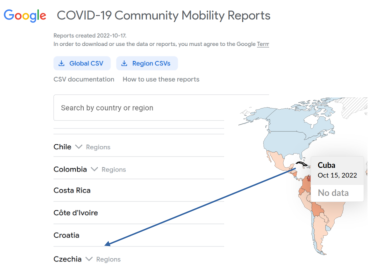
\includegraphics[width=1\textwidth]{Graphics/google_exclusion.pdf} \caption{Cuba excluida por Google en el acceso a modelos de movilidad} \label{fig:google_exclusion}
\end{figure}

Si bien los modelos de movilidad generados por el Centro de Sistemas Complejos, de acuerdo con ETECSA, fueron de gran utilidad, es importante señalar que dichos datos tienen menos precisión y son menos abundantes que los que disponen empresas como Google, Facebook y otras.

Una de las enseñanzas de la pandemia y de la posterior aplicación de estos datos al estudio de la movilidad poblacional es que no se puede esperar a tener situaciones críticas para decidirse a usar estos métodos de análisis de datos. Esencialmente, aunque el posible uso y valor de estos datos sea bastante obvio, en los detalles de cómo extraer valor informacional radica un gran reto. Es importante crear una base científica y tecnológica que permita, ante necesidades concretas, saber las potencialidades de estos datos, si permiten o no enfrentar la tarea en cuestión, y la precisión de los mismos.

\subsection{Estudios cubanos relacionados}

La investigación en Cuba sobre el uso de datos de telefonía móvil para análisis de movilidad y aplicaciones epidemiológicas ha experimentado avances significativos en los últimos años. Roger \cite{casimiro2019movilidad} sentó las bases al desarrollar un sistema informático para procesar registros de llamadas en colaboración con ETECSA, generando matrices origen-destino a escala nacional y demostrando su utilidad en modelación de epidemias. Posteriormente, Orlando \cite{durive2021sistema} profundizó en la extracción de indicadores de movilidad mediante herramientas de inteligencia artificial, desarrollando el \textit{software} BDPhoneFlow, y analizó el impacto de las medidas sanitarias durante la COVID-19. Lius Padrón \cite{padron2021transporte} validó el uso de datos de LAU para identificar disparidades temporales en flujos de movilidad, destacando el efecto del escalonamiento de horarios como medida socioeconómica.

En el ámbito epidemiológico, Alejandro Castro \cite{castro2023movilidad} exploró la relación entre matrices de movilidad derivadas de telefonía y casos de COVID-19 en La Habana, revelando limitaciones en la predictibilidad debido a la preponderancia de contagios intra-área. Por su parte, Andy \cite{rodriguez2022movilidad} abordó específicamente el completamiento de puntos intermedios en trayectorias mediante un modelo de redes neuronales, implementando experimentos en entornos urbanos artificiales y extendiendo su aplicación a datos reales de La Habana. Ernesto \cite{ortega2022modelacion} complementó estos esfuerzos con modelos de física estadística, evaluando la eficacia del rastreo de contactos en Cuba durante la pandemia y destacando el papel crítico de las pruebas masivas.

Aunque estos trabajos han establecido metodologías valiosas, aún existen varios desafíos pendientes, entre ellos el completamiento preciso de trayectorias individuales integrando patrones espaciotemporales complejos en modelos predictivos. Estas limitaciones resaltan la necesidad de enfoques innovadores que combinen el conocimiento local con arquitecturas avanzadas de aprendizaje automático.

\section{Contribución de esta investigación}

Esta investigación propone la aplicación de TrajBERT para el completamiento de trayectorias a partir de datos de telefonía móvil en Cuba. A diferencia de trabajos anteriores que priorizaron el análisis estadístico sobre patrones de movilidad colectiva (matrices origen-destino), esta tesis se centra en reconstruir trayectorias a nivel de usuario individual, un desafío técnicamente más complejo y menos explorado en Cuba. TrajBERT se orienta al completamiento de trayectorias implícitas sin requerir información adicional, como velocidad, condiciones climáticas u otras variables contextuales. Estas características coinciden con la naturaleza de los registros de telefonía en Cuba, lo que hace que este modelo resulte especialmente idóneo para su aplicación en dicho contexto.

Al aplicar una arquitectura basada en \textit{transformers}, se espera superar la efectividad del estudio previo basado en redes neuronales tradicionales \cite{rodriguez2022movilidad}, al tratar las trayectorias como secuencias de ubicaciones interrelacionadas en el espacio y el tiempo, logrando una comprensión más exacta de los patrones de movilidad. Este enfoque promete captar de manera más precisa las dependencias espaciotemporales, posibilitando un completamiento robusto incluso en escenarios con datos escasos y de baja densidad.
\chapter{Validación de TrajBERT como Metodología}\label{chapter:proposal}

En este capítulo, se aborda la implementación práctica del modelo TrajBERT \cite{si2023trajbert}, explorando sus fortalezas y limitaciones en el completamiento de trayectorias humanas. Para ello, se detalla el proceso de diseño e implementación del modelo, desde el preprocesamiento de los datos hasta la configuración de su arquitectura. Adicionalmente, se evalúan las capacidades técnicas de TrajBERT mediante su aplicación a la base de datos pública \textit{HuMob Challenge} 2023 \cite{humob2023}, lo que permite obtener una línea base de desempeño antes de su adaptación a las particularidades del contexto cubano.

El desarrollo de este capítulo se estructura de la siguiente manera: primero, se incluye una definición formal del problema a resolver y se describe la arquitectura y los fundamentos del modelo TrajBERT, destacando sus componentes clave y las razones de su elección para este estudio. A continuación, se presenta el preprocesamiento de los datos y las métricas de evaluación utilizadas para medir el desempeño del modelo. Finalmente, se analizan los resultados obtenidos en esta etapa inicial de implementación, estableciendo una base para las adaptaciones posteriores en el contexto local que serán abordadas en el siguiente capítulo.

\section{Caracterización del modelo}

El modelo TrajBert fue desarrollado por Si et al. en \cite{si2023trajbert} en enero del 2023, para abordar el problema de completamiento de trayectorias humanas. Este modelo destaca por su capacidad para aprender patrones de movilidad de manera bidireccional, refinando las predicciones a través de un proceso de combinación con puntos vecinos conocidos en la trayectoria e incorporando una novedosa función de pérdida consciente del espacio y el tiempo. En los experimentos realizados en \cite{si2023trajbert} sobre conjuntos de datos del mundo real, TrajBERT demostró una mejora de al menos un 8.2\% en comparación con los métodos más avanzados de recuperación de trayectorias disponibles hasta la fecha. Además, en contextos de extrema escasez de datos, como el caso cubano, destacó por su potencial como una herramienta práctica y efectiva en el análisis de la movilidad humana.

\subsection{Preliminares}

Las trayectorias sin procesar son dispersas, no uniformes y presentan variabilidad en el tamaño de la secuencia. Por tanto, en \cite{si2023trajbert} se consideró fundamental partir de una definición formal del problema a resolver. Las definiciones relacionadas se presentan a continuación.

\begin{definition}{ID de Ubicación:}
    Un ID de ubicación corresponde a una región geográfica pero carece de información geográfica explícita, como coordenadas. Puede ser un ID de celda de una estación base, un ID único de Wi-Fi o un identificador único universal (UUID) generado por un generador de números aleatorios.
\end{definition}

\begin{definition}{Trayectoria Implícita:}
    Una trayectoria implícita $T$ se define como una secuencia ordenada temporalmente de IDs de ubicación generada dentro de un día, representada como $T = \{p_1, p_2, \ldots, p_j, \ldots, p_n\}$, donde $p_j$ es el $j$-ésimo punto de la trayectoria, representado como $p_j = (\loc_j, \text{ts}_j)$, siendo $\loc_j$ el ID de ubicación, $\text{ts}_j$ la marca temporal cuando se registró el punto de la trayectoria, y $n$ el número total de puntos registrados.
\end{definition}

\begin{definition}{Trayectoria Muestreada con Intervalo $\epsilon$:}
    Una trayectoria muestreada con intervalo $\epsilon$ se representa como $T_\epsilon = \{\loc_1, \loc_2, \ldots, \loc_j, \ldots, \loc_m\}$, donde $m$ es el número total de intervalos de muestreo en un día. El valor $\epsilon$ es el intervalo de muestreo, es decir, la diferencia de tiempo entre IDs de ubicación consecutivos. La definición del valor de $\epsilon$, así como el tamaño de la ventana de tiempo que se analizará, definirá la cantidad máxima de IDs de ubicación efectivas en una trayectoria. Si falta el ID de ubicación en un intervalo de muestreo $j$, $\loc_j$ será reemplazado por un signo predefinido \emph{PAD}.
    \label{def:e_sampling}
\end{definition}

Finalmente, dada una trayectoria implícita $T$ no uniforme, el \textbf{objetivo} del modelo es recuperarla para obtener una trayectoria muestreada con intervalo $\epsilon$, $T_\epsilon$, prediciendo los IDs de ubicación de los intervalos de muestreo faltantes de manera que se asemeje lo más posible a la ruta de movimiento real del usuario.

\subsection{Arquitectura}

Inspirados por el éxito del modelo BERT \cite{devlin2018bert} en el procesamiento de lenguaje natural, el modelo TrajBERT utiliza el \textit{encoder} de \cite{vaswani2017attention} como red base y el enfoque de \textit{Masked Language Model} (MLM) para su entrenamiento. La idea principal es que si BERT es capaz de completar palabras faltantes en una oración, una arquitectura similar que aproveche los datos espaciotemporales, podrá completar satisfactoriamente puntos faltantes en una trayectoria. Su arquitectura, reflejada en la figura \ref{fig:trajbert_architecture}, consta de tres componentes principales: una capa de preprocesamiento que transforma las trayectorias implícitas, escasas y no uniformes en trayectorias uniformes con muestreo $\epsilon$; un codificador de trayectorias que aprende las representaciones ocultas de las ubicaciones faltantes utilizando el codificador de \textit{transformers} y un esquema de refinamiento espaciotemporal; y una capa de salida diseñada para predecir las ubicaciones faltantes, incorporando dependencias espaciales y temporales mediante una función de pérdida. Estos módulos trabajan de manera conjunta para abordar el problema de recuperación de trayectorias humanas con alta precisión.

\begin{figure}[!htb] \centering 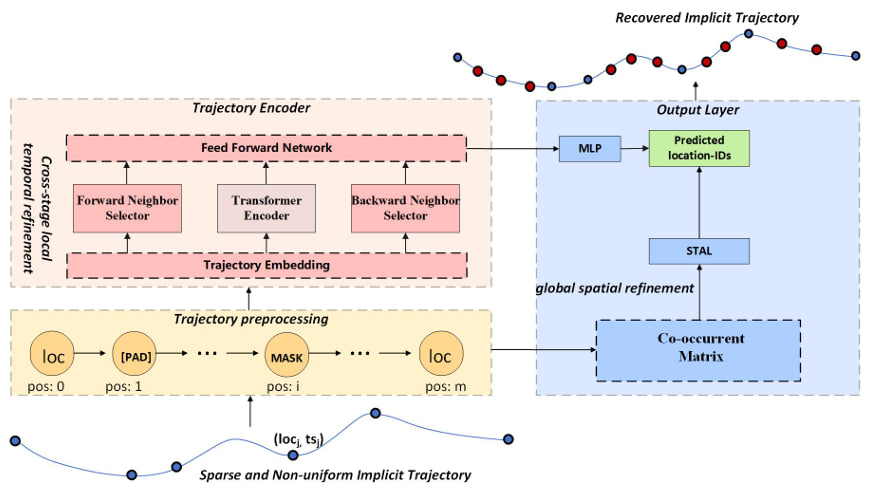
\includegraphics[width=1\textwidth]{Graphics/trajbert_architecture.jpg} \caption{Arquitectura de TrajBERT, figura extraída de \cite{si2023trajbert}.} \label{fig:trajbert_architecture} 
\end{figure}

\subsubsection{Preprocesador de trayectorias}

El problema de recuperación de trayectorias enfrenta importantes desafíos debido a la naturaleza no uniforme y de longitud variable de las trayectorias, que presentan patrones de movilidad con granularidades diversas y brechas temporales entre registros consecutivos que pueden variar desde segundos hasta horas. Para abordar esta problemática, en \cite{si2023trajbert} proponen transformar las trayectorias implícitas originales en trayectorias con muestreo $\epsilon$, permitiendo trabajar con entradas de longitud fija. En este enfoque, cada trayectoria se segmenta en intervalos temporales basados en la marca de tiempo (\textit{timestamp}) de cada punto, como se detalla en la ecuación ~\ref{eq:segments}:

\begin{equation}
\text{seg}_i = \cup \{ \loc_j \mid \text{ts}_j \% 86400 / \epsilon = i \}
\label{eq:segments}
\end{equation}

\noindent
donde $i$ representa el $i$-ésimo intervalo de tiempo, $\text{seg}_i$ corresponde al segmento de trayectoria dentro de ese intervalo, y $\epsilon$ define la duración de cada intervalo de tiempo. 

En el caso de intervalos con múltiples valores de \textit{ID de ubicación}, los autores seleccionan el valor más frecuente como representante. Para los intervalos sin registros, se introduce un signo predefinido de \textit{padding} (\textit{‘PAD’}). Finalmente, estas trayectorias con muestreo $\epsilon$ se representan como $T_\epsilon = \{\loc_1, \loc_2, \cdots, \loc_j, \cdots, \loc_m\}$, sirviendo como entradas para la capa de codificación de trayectorias.

\subsubsection{Codificador de trayectorias}
\label{trajectory_encoder}

Según lo descrito por los autores en \cite{si2023trajbert}, la recuperación de trayectorias comparte similitudes con el \textit{cloze task}\footnote{El \textit{cloze task} es un método de evaluación que mide la habilidad de los participantes para completar un texto que contiene palabras omisas, asegurando la comprensión contextual de la información presentada.} en el procesamiento de lenguaje natural. Ambas requieren predecir elementos faltantes (tokens o \textit{ID de ubicación}) utilizando información anterior y posterior en la secuencia. En este caso, el objetivo es definir una función de mapeo $f$ para predecir el \textit{ID de ubicación} del $i$-ésimo intervalo de tiempo, con base en las trayectorias con muestreo $\epsilon$ como entrada, de forma que ${pred\_loc}_i = f(i, T_\epsilon)$.

Para lograrlo, se emplea el \textit{encoder} de \textit{transformers} junto con un esquema de refinamiento espaciotemporal. Este codificador bidireccional utiliza un mecanismo de atención multi-cabeza, lo que permite considerar puntos de la trayectoria en ambas direcciones y modelar de manera efectiva patrones de movilidad espaciotemporales. Durante el entrenamiento, los autores aplican la técnica de enmascaramiento propuesta en BERT, donde un 15\% de los \textit{ID de ubicación} efectivos se enmascaran aleatoriamente, omitiendo los intervalos marcados como ‘PAD’. Los \textit{ID de ubicación} enmascarados se configuran como ‘MASK’ con un 80\% de probabilidad, se mantienen igual en un 10\% y como un \textit{ID de ubicación} aleatorio en el 10\% restante.

Para alimentar las trayectorias al \textit{encoder}, se convierten los \textit{ID de ubicación} y los índices de los intervalos de tiempo en representaciones densas mediante una capa de \textit{embeddings} entrenable. Estos \textit{embeddings} se combinan con codificaciones posicionales para formar los vectores de entrada:

\begin{equation}
E_{T_\epsilon} = E_{\loc} + E_{\text{pos}}
\end{equation}

El \textit{encoder} utiliza múltiples capas con mecanismos de atención para aprender patrones espaciotemporales bidireccionales y cada capa aplica normalización, redes de avance y activaciones \textit{Gelu} \cite{lee2023gelu} para generar representaciones ocultas de las trayectorias.

Para mejorar la precisión en la recuperación de trayectorias, los autores diseñan un esquema de refinamiento espaciotemporal que enfatiza los \textit{ID de ubicación} vecinos recientemente visitados y próximos por visitar. Si bien el mecanismo de atención ya captura dependencias contextuales a lo largo de la secuencia, este enfoque introduce un ajuste adicional independiente del \textit{encoder} para mitigar posibles sesgos y mejorar el completamiento de puntos faltantes. Para ello, incorpora vectores de \textit{embedding} de los vecinos más cercanos hacia adelante y hacia atrás, combinándolos con las representaciones vectoriales ocultas aprendidas por el \textit{encoder}. Esta estrategia representa el primer aporte de \cite{si2023trajbert} al campo del completamiento de trayectorias, basado en la hipótesis de que los puntos más influyentes sobre un token faltante son sus vecinos inmediatos en ambas direcciones.

\subsubsection{Capa de salida}
\label{stal_function}

\begin{wrapfigure}{r}{0.6\textwidth}
  \centering
  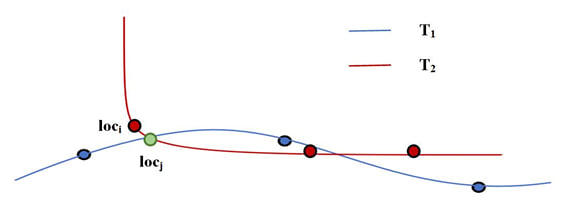
\includegraphics[width=0.5\textwidth]{Graphics/co_ocurrent_trajectories.jpg}
  \caption{$loc_i$ y $loc_j$ co-ocurren frecuentemente, son espacial y temporalmente contiguos, figura extraída de \cite{si2023trajbert}}
  \label{fig:co_ocurrent_trajectories}
\end{wrapfigure}

La capa de salida de TrajBERT introduce una novedosa función de pérdida para incorporar dependencias espaciales globales en el entrenamiento del modelo. 
Si dos \textit{ID de ubicación} (\(\loc_i\) y \(\loc_j\)) co-ocurren frecuentemente en trayectorias, se consideran contiguos tanto espacial como temporalmente, representando áreas geográficamente cercanas. Por ejemplo, en \ref{fig:co_ocurrent_trajectories} el punto $loc_j$ de $T_1$ co-ocurre frecuentemente con $loc_i$ en otras trayectorias, ambos puntos son cercanos geográficamente. A partir de esta relación de co-ocurrencia, se construye una matriz \(H\), definida como:

\begin{equation}
H[\loc_i][\loc_j] = \frac{co_{\loc_i, \loc_j}}{\sum_{l} co_{\loc_i, l}},
\label{eq:co_ocurrence_matrix}
\end{equation}

\noindent
donde \(co_{\loc_i, \loc_j}\) es el valor de co-ocurrencia entre \(\loc_i\) y \(\loc_j\).

La salida del modelo asigna a cada \textit{ID de ubicación} posible una probabilidad, la cual es inicialmente optimizada mediante una función de pérdida estándar basada en entropía cruzada (\textit{Cross Entropy Loss}, \(CEL\)). Sin embargo, esta función no diferencia entre predicciones geográficamente cercanas y lejanas al valor real, lo que puede resultar en penalizaciones injustas para predicciones que representan ubicaciones cercanas al objetivo real.

Para abordar este problema, \cite{si2023trajbert} propone una función de pérdida consciente del espacio y tiempo (\textit{Spatial-Temporal Aware Loss}, \(\text{STAL}\)), que incorpora las estructuras espaciales globales aprendidas de la matriz \(H\). \(\text{STAL}\) está definida como:

\begin{equation}
\text{STAL} = \beta_1 \cdot L_1 + \beta_2 \cdot L_2,
\label{eq:stal}
\end{equation}

\noindent
donde $ \beta_1$ y $ \beta_2$ son hiperparámetros que balancean la optmización de STAL, \(L_1\) se calcula por las ecuaciones \ref{eq:l_1}  y \ref{eq:stal_sigma} y \(L_2\) es el CEL:

\begin{equation}
    L_1 = - \sum_{i=1}^N \sum_{j=1}^M \sum_{k=1}^S \sigma_{i,j,k} \log \left( P(\loc_{i,j,k} \mid T^\epsilon_i, \theta) \right),
\label{eq:l_1}
\end{equation}

\begin{equation}
    \sigma_{i,j,k} = \left( 1 - P(t_{i,j} \mid T^\epsilon_i, \theta) \right) \cdot \left( 1 - w(t_{i,j}, \loc_{i,j,k}) \right),
\label{eq:stal_sigma}
\end{equation}

\noindent
donde \(w(loc_i, loc_j)\) es el coeficiente espaciotemporal entre el \textit{ID de ubicación} real y el que se quiere predecir:

\begin{equation}
    w(\loc_i, \loc_j) =
    \begin{cases} 
        1, & \text{si } \loc_i = \loc_j, \\
        \displaystyle \frac{\exp(H[\loc_i][\loc_j] / \mu)}{\sum_s \exp(H[\loc_i][\loc_s] / \mu) + \eta}, & \text{si } H[\loc_i][\loc_j] > \gamma, \\
        0, & \text{en otro caso.}
    \end{cases}
\label{eq:w_loc_cases}
\end{equation}

\noindent
aquí, \(\gamma\) es un umbral de co-ocurrencia, \(\mu\) es un parámetro de escala y \(\eta\) es una constante. Esta función de pérdida reduce las penalizaciones para predicciones cercanas geográficamente al valor real, alineándose con las restricciones de movilidad humana impuestas por las estructuras espaciales de las ciudades.

\subsection{Implementación}

El modelo se reimplementó utilizando Python 3.12.4 y PyTorch (2.3.1+cu118) y se basó en un repositorio público disponible en \href{https://github.com/TrajResearch/TrajBERT}{GitHub} \cite{trajebert_repo}, que sirvió como punto de partida para este trabajo. No obstante, no hay certeza de que dicho repositorio pertenezca oficialmente a los autores del artículo, ya que en el texto no se hace referencia a este. Sin embargo, una de las colaboradoras del repositorio incluye su dirección de correo electrónico, la cual coincide con el nombre de una de las autoras del artículo, lo que sugiere una posible relación entre ambos. Además, el código del repositorio implementa de manera consistente la arquitectura descrita en el artículo, lo que refuerza la idea de que está directamente basado en la propuesta original.

Sin embargo, el código original presentaba múltiples desafíos que requerían una revisión profunda y adaptaciones significativas para ajustarse a los objetivos del estudio. La falta de documentación en el repositorio dificultaba la comprensión del flujo general del modelo, por lo que fue necesario analizar minuciosamente cada componente del código para comprender su funcionalidad.

Otro desafío importante fue que la arquitectura del modelo estaba diseñada para recibir un formato muy específico de datos, ver apéndice  \ref{apx:trajbert_data_format}, por lo que fue imprescindible establacer protocoles de conversión sobre los datos utilizados para no cambiar el código fuente del modelo. Además, se eliminaron secciones del código que resultaban innecesarias, ya que no influían en el flujo del modelo. Se optimizó el tiempo de ejecución de ciertos procesos mediante la incorporación de operaciones vectoriales con la biblioteca NumPy, específicamente en la construcción de la matriz de co-ocurrencia, ver apéndice \ref{apx:source_code_modified}. Durante la implementación se realizaron pruebas exhaustivas, tanto unitarias como con datos reales, para garantizar la robustez del sistema, corregir errores que no estaban contemplados en el diseño original y garantizar la coherencia en los resultados. Por ejemplo, el código original no permitía que la cantidad de ubicaciones enmascaradas en trayectorias analizadas en un mismo lote fuera variable, lo cual impedía enmascarar una cantidad de ubicaciones proporcional a la cantidad de ubicaciones conocidas. Por tanto, fue necesario implementar un mecanismo de relleno dinámico mediante una función de colación personalizada, que ajusta automáticamente las secuencias de entrada y genera máscaras binarias, permitiendo procesar lotes con trayectorias de distinta longitud sin afectar la estructura del modelo, ver apéndice \ref{apx:dynamic_padding}. Finalmente, para evaluar todos los modelos generados durante el entrenamiento, se implementó un procedimiento automatizado que carga cada modelo, ejecuta la inferencia sobre un conjunto de prueba y almacena los resultados. Para una descripción detallada de esta implementación, véase el apéndice \ref{apx:evaluate_all_models}.

Finalmente, se mejoró la documentación del código, incluyendo comentarios detallados y explicaciones de los parámetros. Este paso no solo facilitó la comprensión del modelo, sino que también permitirá reutilizar y expandir su funcionalidad en futuros trabajos. El proceso de implementación fue una adaptación profunda y consciente que involucró modificaciones técnicas y mejoras en la eficiencia, lo que resultó en un modelo funcional, optimizado y alineado con los objetivos de este trabajo. La implementación de este trabajo fue también puesta a disposición de la comunidad en \url{https://github.com/alexsierra45/thesis/tree/main/src/trajbert}.

\subsection{Opinión del autor}

El modelo TrajBERT presenta una arquitectura robusta y bien diseñada para el completamiento de trayectorias y reconocimiento de patrones humanos. Su enfoque basado en \textit{transformers}, combinado con el refinamiento espaciotemporal y la función STAL, suponen una solución prometedora en contextos donde la información disponible es limitada.

Sin embargo, desde el punto de vista de su diseño, TrajBERT presenta algunas limitaciones que mitigan el valor contextual que ofrecen otros datos relativos a las trayectorias. En primer lugar, no está diseñado para aprovechar el conocimiento sobre qué usuario realizó cada trayectoria, lo cual restringe la capacidad del modelo para personalizar las predicciones o identificar patrones específicos de usuarios individuales. En segundo lugar, la arquitectura no considera información temporal como el día de la semana, lo que podría ser crucial para detectar patrones periódicos en los datos, como trayectorias relacionadas con rutinas laborales o actividades recreativas recurrentes. Además, una tercera limitación es la omisión de variables ambientales y contextuales, como las condiciones climáticas o los medios de transporte empleados, factores que pueden influir notablemente en la dinámica y elección de los desplazamientos. Por último, el modelo no incorpora explícitamente el papel de los puntos de interés en las distintas zonas geográficas, lo que podría ser relevante para entender las motivaciones detrás de las trayectorias y capturar relaciones espaciales significativas en los datos.

Dado que TrajBERT se centra en el modelado de trayectorias implícitas, su diseño enfatiza la secuencialidad de los \textit{ID de ubicación} dentro de un mismo día, sin incorporar explícitamente información contextual como la identidad anonimizada del usuario o la relevancia de puntos de interés específicos. Por tanto estas observaciones no se basan en ningún experimento en particular, sino en un análisis teórico de la arquitectura. Sin embargo, la incorporación de estos factores no garantiza de manera inmediata un mejor entendimiento de la movilidad urbana, pero plantea una rama de investigación interesante respecto a hasta qué punto estos datos contextuales podrían influir en un modelo que analiza trayectorias como secuencias espaciotemporales. Se podrían formular nuevas preguntas, tales como: ¿Cómo afecta la incorporación de datos contextuales la precisión en el completamiento de trayectorias? ¿Qué impacto tienen factores externos, como el clima o los patrones de transporte, en la predicción de rutas en entornos urbanos? ¿Es posible diseñar mecanismos de fusión de información que integren estos datos de forma eficiente sin incrementar excesivamente la complejidad del modelo? Estas interrogantes abren la puerta a explorar nuevos horizontes en el análisis de la movilidad, lo que posibilita desarrollar modelos más sensibles a las particularidades de cada entorno.

\section{Evaluación de TrajBERT en datos de \textit{HuMob} 2023}

En esta sección, se describe la implementación de TrajBERT sobre un conjunto de datos real proveniente de la competencia \textit{HuMob} en su edición del 2023 \cite{humob2023}. Inicialmente, se presentan las principales estadísticas de los datos, destacando los factores que influyeron en las decisiones tomadas durante el proceso de diseño y entrenamiento del modelo. Posteriormente, se analizan los resultados obtenidos en los experimentos realizados, comparando el desempeño de TrajBERT con enfoques tradicionales. Finalmente, se discuten las conclusiones obtenidas, resaltando las ventajas de esta arquitectura en contextos reales.

\subsection{Humob \textit{challenge}}

El \textit{Human Mobility (HuMob) Challenge} \cite{humob2023} es una competencia internacional que busca evaluar y mejorar los modelos computacionales para la predicción de patrones de movilidad humana. Utilizando conjuntos de datos abiertos y de gran escala, que reflejan trayectorias de movimiento humano en áreas metropolitanas, este desafío proporciona a los investigadores una plataforma estandarizada para desarrollar y probar sus métodos de predicción. Los participantes reciben datos de movimiento de individuos durante un período determinado, segmentados en intervalos de 30 minutos. El objetivo es predecir los movimientos de un subconjunto de individuos en ciertas ciudades durante días específicos, utilizando datos históricos de movimiento tanto de la misma ciudad como de otras.

Para facilitar el desarrollo de modelos de predicción, se proporciona información adicional sobre los puntos de interés (\textit{Points of Interest}, POI) en cada celda de la cuadrícula, representada por vectores de múltiples dimensiones. Aunque las categorías específicas de los POI no se divulgan, esta información puede ser útil para capturar patrones de movilidad relacionados con la infraestructura urbana. La evaluación de las predicciones se realiza comparando las trayectorias previstas con las reales, utilizando métricas como GEO-BLEU \cite{shimizu2022geo} y \textit{Dynamic Time Warping} (DTW) \cite{muller2007dynamic}. Estas métricas permiten medir la precisión de las predicciones desde diferentes perspectivas, considerando tanto la similitud local como la alineación temporal de las trayectorias. 

El \textit{HuMob Challenge}, como iniciativa internacional centrada en la modelación de movilidad humana, ofrece un marco de referencia valioso al proporcionar datos estandarizados y protocolos de evaluación comparables. Si bien su enfoque original difiere del objetivo de este trabajo de completar trayectorias implícitas a partir de secuencias diarias, la riqueza del conjunto de datos permite evaluar las capacidades base de TrajBERT en condiciones cercanas a escenarios reales. 

Es crucial señalar que las métricas utilizadas en la competencia, diseñadas para evaluar la precisión de las predicciones, no capturan completamente los requisitos del presente enfoque, que prioriza la identificación de patrones macroespaciales y admite márgenes de error geográfico más amplios. Esta metodología aprovecha el valor comparativo de la competencia, reconociendo sus particularidades sin establecer comparaciones directas, lo que permite una adaptación más informada del modelo a problemáticas específicas de movilidad en contextos con recursos limitados.

\subsection{Conjunto de datos}

El conjunto inicial de datos fue curado mediante un recorte espacial y temporal de datos brutos de telefonía móvil. Se definió un área delimitada alrededor de una ciudad en Japón, seleccionando usuarios que fueron observados dentro de esta área al menos 10 veces durante un período de 10 días. Para preservar el anonimato, las ubicaciones se discretizaron en celdas de 500 m × 500 m, los tiempos se agruparon en intervalos de 30 minutos y las fechas exactas se enmascararon. Los datos registran el movimiento de los usuarios durante 60 días de actividad normal y 15 días durante una situación de emergencia. Solo se incluyeron usuarios con un número suficiente de observaciones, resultando en 25,000 usuarios. Las observaciones fuera del área delimitada fueron descartadas. En este estudio solo se usaron los primeros 5,000 usuarios y las trayectorias de sus primeros 60 días de actividad normal. 

\begin{figure}[!htb]
\centering
\begin{minipage}{0.5\textwidth}
    \centering
    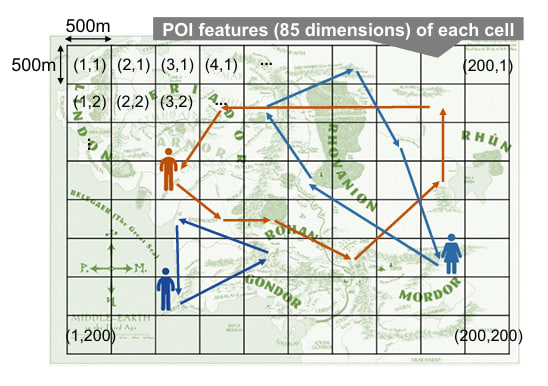
\includegraphics[width=\textwidth]{Graphics/humob_matrix_mobility.jpg}
    \caption{Las trayectorias fueron discretizadas en celdas de 500 m × 500 m en una matriz de 200 x 200 celdas, figura extraída de \cite{yabe2024yjmob100k}.}
    \label{fig:humob_matrix_mobility}
\end{minipage}%
\hfill
\begin{minipage}{0.45\textwidth}
    \centering
    \begin{tabular}{|c|c|c|c|c|}
    \hline
    \textbf{uid} & \textbf{d} & \textbf{t} & \textbf{x} & \textbf{y} \\ \hline
    1 & 10 & 31 & 7 & 10 \\ \hline
    1 & 10 & 32 & 7 & 10 \\ \hline
    1 & 10 & 33 & 8 & 9  \\ \hline
    1 & 10 & 34 & 9 & 13 \\ \hline
    1 & 10 & 35 & 8 & 8  \\ \hline
    1 & 10 & 37 & 8 & 8  \\ \hline
    1 & 10 & 38 & 7 & 8  \\ \hline
    \multicolumn{5}{|c|}{\dots} \\ \hline
    \end{tabular}
    \captionof{table}{Ejemplo de los datos del conjunto de usuarios y sus ubicaciones discretizadas.}
    \label{tab:humob_example_data}
\end{minipage}
\end{figure}

La tabla \ref{tab:humob_example_data} muestra un ejemplo del conjunto de datos proporcionado. Cada registro representa una observación de un individuo y consta de las siguientes columnas:

\begin{itemize}
    \item El ID de usuario es un identificador único para cada usuario de teléfono móvil.
    \item El día corresponde a la fecha enmascarada de la observación, que puede variar entre 0 y 59.
    \item El intervalo de tiempo representa la marca temporal discretizada en intervalos de 30 minutos, con valores entre 0 y 47; por ejemplo, 0 indica el intervalo entre las 00:00 y 00:30 horas, mientras que 13 corresponde al intervalo entre las 6:30 y 7:00 horas.
    \item Las coordenadas x, y indican la ubicación observada mapeada en una cuadrícula discretizada de 500 metros, con valores que van de (1, 1) a (200, 200), como se ilustra en la figura \ref{fig:humob_matrix_mobility}.
\end{itemize}

El número total de registros es 4,999,742 entre los 5,000 usuarios. La figura \ref{fig:unique_cell_per_user_histogram} muestra un histograma del número de celdas únicas visitadas por usuarios, se visualiza una distribución sesgada, donde una pequeña fracción de los usuarios es observada muchas veces. La figura \ref{fig:unique_user_per_cell_histogram} muestra el histograma del número de usuarios únicos que visitaron cada celda, el eje x está en escala logarítmica. El gráfico muestra que una fracción de las celdas son visitadas muy pocas veces (menos de 10 usuarios únicos), mientras que se puede observar otra acumulación alrededor de los 100 usuarios únicos, lo cual resalta la mezcla de áreas urbanas y rurales en la región estudiada.

\begin{figure}[!htb]
\centering
\begin{minipage}{0.45\textwidth}
    \centering
    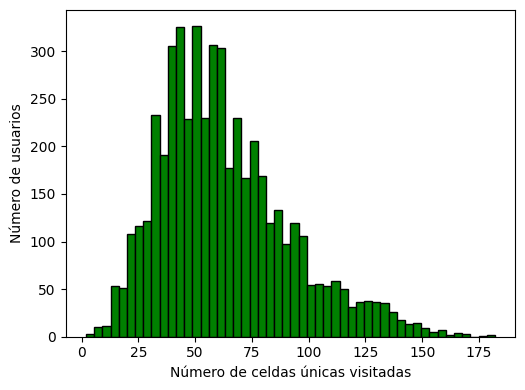
\includegraphics[width=\textwidth]{Graphics/unique_cell_per_user_histogram.png}
    \caption{Histograma del número de celdas únicas visitadas por usuarios.}
    \label{fig:unique_cell_per_user_histogram}
\end{minipage}%
\hfill
\begin{minipage}{0.45\textwidth}
    \centering
    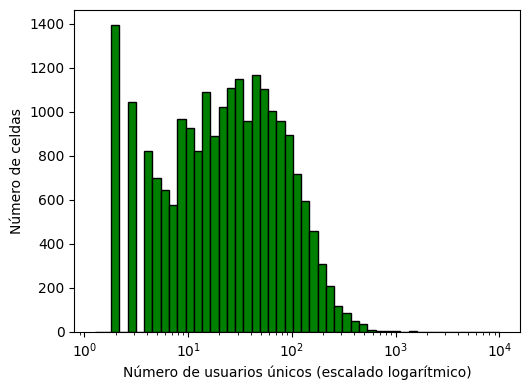
\includegraphics[width=\textwidth]{Graphics/unique_user_per_cell_histogram.png}
    \caption{Histograma del número de usuarios únicos por celdas.}
    \label{fig:unique_user_per_cell_histogram}
\end{minipage}%
\end{figure}

La figura \ref{fig:unique_user_per_day_plot} muestra la dinámica temporal del número usuarios únicos por día desde el día 0 hasta el 59. Los patrones muestran regularidad temporal, con patrones claros de días laborables y fines de semana. Hay una anomalía en el día 27, por tanto fueron excluidos del análisis los registros de ese día. La figura \ref{fig:ping_per_timeslot_plot} muestra la dinámica temporal del número de registros por intervalo de tiempo desde el intervalo 0 hasta el 47, agregados a lo largo de todos los días. Los patrones muestran regularidad temporal, con picos claros en la mañana, la tarde y al mediodía.

\begin{figure}[!htb]
\centering
\begin{minipage}{0.45\textwidth}
    \centering
    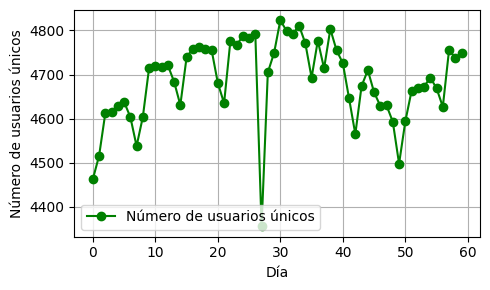
\includegraphics[width=\textwidth]{Graphics/unique_user_per_day_plot.png}
    \caption{Dinámica temporal del número de usuarios únicos por día.}
    \label{fig:unique_user_per_day_plot}
\end{minipage}%
\hfill
\begin{minipage}{0.45\textwidth}
    \centering
    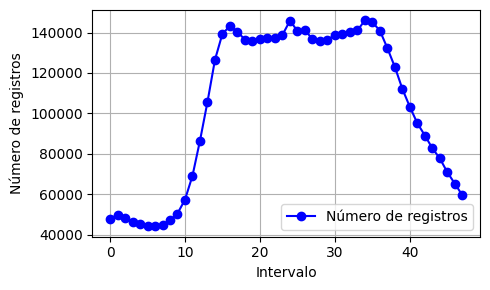
\includegraphics[width=\textwidth]{Graphics/ping_per_timeslot_plot.png}
    \caption{Dinámica temporal del número de registros por intervalo, agregados a lo largo de todos los días.}
    \label{fig:ping_per_timeslot_plot}
\end{minipage}%
\end{figure}

La figura \ref{fig:unique_user_per_cell_2_dimensional_histogram} (izquierda) muestra un histograma bidimensional en escala logarítmica del número de usuarios únicos por celda observados a lo largo de los 60 días de estudio. Los patrones muestran claramente áreas urbanas y rurales. Finalmente, se realizó una reducción de resolución al mapa de trayectorias discretizadas de 200 × 200 a 20 × 20, como se puede ver en la figura \ref{fig:unique_user_per_cell_2_dimensional_histogram} (derecha), lo cual disminuye significativamente el costo computacional al reducir el número de celdas de 40,000 a 400, optimizando recursos y tiempos de ejecución, mientras preserva los patrones globales de densidad de usuarios y registros al sumar los valores agrupados, manteniendo la representatividad del comportamiento general.

\begin{figure}[!htb] \centering 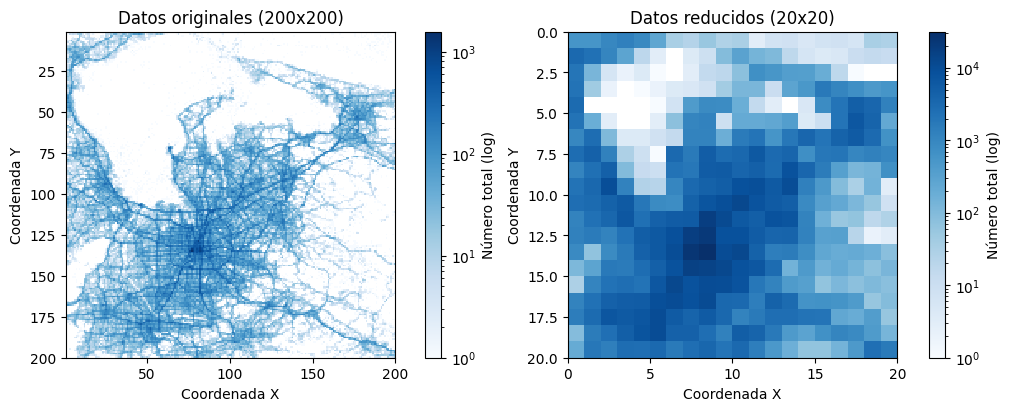
\includegraphics[width=1\textwidth]{Graphics/unique_user_per_cell_2_dimensional_histogram.png} \caption{Histograma bidimensional del número de usuarios únicos por celda. Datos originales a la izquierda, reducidos a la derecha.} \label{fig:unique_user_per_cell_2_dimensional_histogram} 
\end{figure}

\subsection{Experimentos y discusión} 
\label{sec:humob_experiments}

El objetivo principal de este experimento es validar la efectividad de la arquitectura propuesta por TrajBERT para el completamiento de trayectorias en un conjunto de datos real, así como examinar el rendimiento de la función de pérdida y del refinamiento espaciotemporal propuesto en \cite{si2023trajbert}, evaluando la robustez del método con diversos grados de escasez de datos.

Para evaluar la superioridad de TrajBERT, se comparó con tres modelos base. El primer par de modelos son heurísticos, basados en conocimiento previo sobre patrones de movilidad humana, mientras que BERT es un modelo típico para procesar datos secuenciales. La descripción de los modelos base es la siguiente:

\begin{itemize}
    \item \textbf{Histórico:} Utiliza las ubicaciones más populares de cada usuario en cada intervalo de tiempo histórico para realizar la recuperación.
    \item \textbf{Top:} Utiliza las ubicaciones más populares de cada usuario a lo largo de todas las trayectorias históricas para realizar la recuperación.
    \item \textbf{BERT:} Se desactiva el refinamiento espaciotemporal y la función STAL de TrajBERT, manteniendo únicamente el codificador \textit{transformers} y el modelo de lenguaje enmascarado (MLM) para recuperar las ubicaciones omitidas.
\end{itemize}

El conjunto de trayectorias fue particionado en conjuntos de entrenamiento, validación y prueba en un 70\%, 15\% y 15\% respectivamente. En cada trayectoria se enmascaró el 15\% de las ubicaciones efectivas. Los valores $\epsilon, m$ definidos en \ref{def:e_sampling} se pusieron en 30 minutos y 48 intervalos respectivamente, haciendo las 24 horas del día. Los hiperparámetros \(\gamma\), \(\mu\) y \(\eta\) de la ecuación \ref{eq:w_loc_cases} se establecieron en 98, 1000 y $exp(1)$. Los valores \(\beta_1\) y \(\beta_2\) de la ecuación \ref{eq:stal} se hicieron iguales a 1. Adicionalmente, la tasa de aprendizaje se estableció en $10^{-4}$, el tamaño del lote en 256, la cantidad de cabezas de atención en 8, la cantidad de capas en 6, el tamaño del \textit{embedding} en 512 y se usó el optimizador Adam. El entrenamiento se llevó a cabo en una laptop Acer Nitro ANV15-51 con Windows 11 Home 64-bit, procesador Intel Core i7-13620H (16 CPUs, ~2.4GHz), 16GB de RAM y equipado con una tarjeta gráfica NVIDIA GeForce RTX 4050.

Para evaluar el rendimiento de recuperación, se emplean las métricas \textbf{top-k}
y la \textbf{media de la distancia de Manhattan}:

\begin{itemize}
    \item \textbf{Top-k:} Si el \textit{ID de ubicación} verdadero aparece dentro de los primeros $k$ resultados predichos, el valor de top-k es 1, de lo contrario, es 0. El top-k final es el cociente entre las predicciones correctas y el total de localizaciones enmascaradas. Para este experimento se reportan valores de top-k con $k=1$ y $k=3$. Para $k=1$ este valor es la exactitud.
    \item \textbf{Distancia de Manhattan:} Es una métrica utilizada para evaluar la proximidad entre las ubicaciones predichas y las ubicaciones reales en términos de su distancia geográfica. Calcula el promedio de las suma de las diferencias absolutas entre las coordenadas de dos puntos (latitud y longitud). Podemos usar esta métrica debido a la forma matricial que tienen nuestros datos (ver figura \ref{fig:humob_matrix_mobility}).
\end{itemize}

Valores más altos de top-k y más bajos en la media de la distancia de manhattan indican un mejor rendimiento del modelo. Además, \cite{si2023trajbert} introduce una métrica llamada \textit{\textbf{fuzzy accuracy} (fuzzy-acc)} para evaluar la capacidad del modelo de recuperar rutas de movimiento reales. La \textit{fuzzy-acc} considera \textit{IDs de ubicaciones} geográficamente cercanas como válidas para evitar penalizaciones innecesarias. La \textit{fuzzy-acc} se define como:

\begin{equation}
    \text{fuzzy-acc} = 
    \begin{cases} 
    1, & \text{si } \text{predicción} \in C_{i,j} \\
    0, & \text{en otro caso}
    \end{cases}
\end{equation}
 
\noindent
donde $C_{i,j}$ es el conjunto de \textit{IDs de ubicación} similares al valor verdadero $t_{i,j}$, definido como:

\begin{equation}
    C_{i,j} = \bigcup \{k \,|\, H[t_{i,j}][k] > \gamma\}
\end{equation}

\noindent
aquí, $H$ es la matriz de co-ocurrencia \ref{eq:co_ocurrence_matrix} de todos los \textit{IDs de ubicación} y $\gamma$ es el umbral de co-ocurrencia usado en la ecuación \ref{eq:w_loc_cases}. 

La tabla \ref{tab:model_comparison} muestra el rendimiento de los modelos base y TrajBERT, con un 15\% de ubicaciones efectivas enmascaradas. El desempeño de los métodos \textbf{Histórico} y \textbf{Top} es bastante limitado debido a su incapacidad de aprender patrones complejos de movilidad, sin embargo la cantidad de datos permitió lograr una exactitud cercana al 40\% en ambos casos. Aunque BERT no fue diseñado específicamente para el completamiento de trayectorias, el experimento evidencia que el uso de la red \textit{feed-forward} y la conexión residual en el \textit{encoder} puede generar resultados satisfactorios.

TrajBERT obtiene mejores resultados que el resto de los modelos base con un margen significativo. Comparado con BERT, TrajBERT mejora el \textit{encoder} de \textit{transformers} mediante el refinamiento espaciotemporal y la función STAL. Por un lado, el refinamiento espaciotemporal refuerza la importancia de los \textit{ID de ubicación} visitados recientemente y por visitar, y por otro lado, la función de pérdida incorpora información espacial global, ya que las trayectorias están restringidas por la topología de la ciudad. Los últimos tres registros de la tabla \ref{tab:model_comparison} presentan resultados que validan el uso del refinamiento espaciotemporal y la función STAL.

\begin{table}[ht]
\centering
\begin{tabular}{|l|c|c|c|c|}
\hline
\textbf{Modelo}             & \textbf{Exactitud} & \textbf{Fuzzy} & \textbf{Top-3} &  \textbf{Manhattan} \\ \hline
Top                         & 0.3924             & -              & -              & -                   \\ \hline
Histórico                   & 0.4162             & -              & -              & -                   \\ \hline
Bert                        & 0.5415             & 0.7927         & 0.5580         & 2.1248              \\ \hline
TrajBert sin ref. es-temp.  & 0.5784             & 0.8776         & 0.6887         & 1.9426              \\ \hline
TrajBert sin STAL           & 0.6021             & 0.8128         & 0.7882         & 1.7268              \\ \hline
TrajBert                    & 0.6104             & 0.9141         & 0.7980         & 1.7044              \\ \hline
\end{tabular}
\captionof{table}{Comparación de resultados de los modelos.}
\label{tab:model_comparison}
\end{table}

Se evaluó la robustez de TrajBERT, ya entrenado, frente a diferentes escenarios de escasez de datos, configurando la tasa de ocultamiento del conjunto de prueba entre 10\% y 90\%, con el objetivo de disminuir la información del contexto y comprobar la capacidad del modelo de recuperar las ubicaciones enmascaradas. La tasa de ocultamiento se define como el número de ubicaciones efectivas ``eliminadas'' intencionalmente sobre el número total de ubicaciones efectivas. La tasa de pérdida se calcula con la siguiente fórmula:

\begin{equation}
\text{Tasa de pérdida} = \frac{n_{\text{mask}} + n_{\text{pad}} + n_{\text{hid}}}{m}
\end{equation}

\noindent
donde $n_{\text{mask}}$ es el número de ubicaciones enmascaradas, $n_{\text{hid}}$ es el número de ubicaciones ocultadass, $n_{\text{pad}}$ es el número de ubicaciones desconocidas y marcadas como \textit{padding}, y $m$ es el total de intervalos de tiempo.

El modelo TrajBERT demostró una notable capacidad de recuperación, manteniendo un rendimiento destacado incluso con tasas de pérdida superiores al 80\%. En estos escenarios, logró predecir correctamente más del 50\% de las ubicaciones enmascaradas, mostrando su eficacia en condiciones de datos altamente escasos. Se puede apreciar el comportamiento de las métricas de evaluación del modelo en la figura \ref{fig:humob_hidden_variability_analisys}. 

\begin{figure}[!htb] 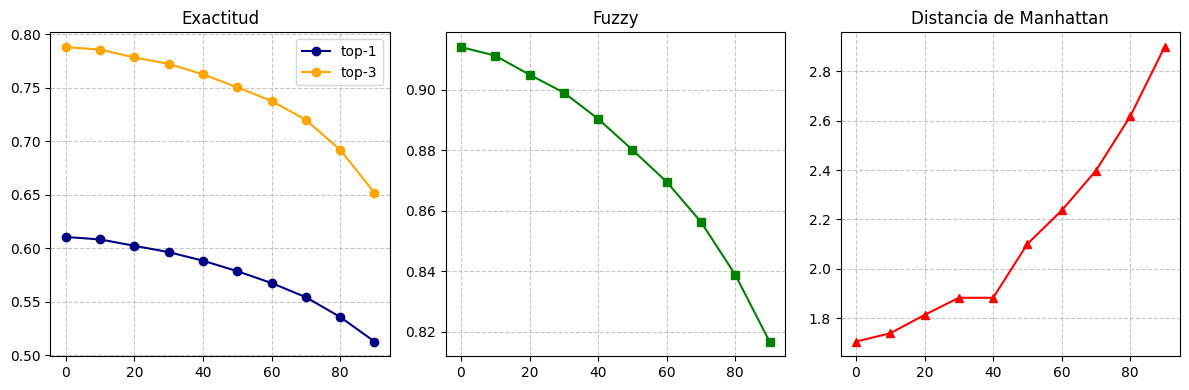
\includegraphics[width=1\textwidth]{Graphics/humob_hidden_variability_analisys.png} \caption{Relación entre el porcentaje de datos ocultos y el desempeño del modelo. Cada gráfico muestra cómo varía una métrica específica al incrementar el nivel de ocultamiento en las trayectorias.} \label{fig:humob_hidden_variability_analisys} 
\end{figure}

Los resultados son los esperados. A medida que aumenta la tasa de ocultamiento, el modelo presenta métricas inferiores, aunque se mantienen en niveles robustos. De aquí se pueden inferir dos ideas interesantes: primero, el rendimiento del modelo es altamente sensible a la información contextual de la secuencia; y segundo, un entrenamiento con una baja tasa de pérdida es capaz de obtener buenos resultados incluso en conjuntos de datos altamente escasos.
\chapter{Completamiento de Trayectorias en La Habana}\label{chapter:implementation}

El presente capítulo tiene como objetivo aplicar el modelo TrajBERT al conjunto de datos de telefonía móvil de Cuba para abordar el problema del completamiento de trayectorias. En particular, se busca inferir puntos faltantes en las trayectorias a partir de datos parciales y explorar su utilidad en este contexto específico.

Para ello, primero se realiza un análisis exploratorio del conjunto de datos, describiendo sus características principales y los desafíos específicos relacionados con trayectorias incompletas. A continuación, se presentan los resultados de la aplicación del modelo, destacando los casos de éxito y los retos encontrados. Por último, se comparan estos resultados con un estudio similar realizado previamente en Cuba, analizando las diferencias metodológicas y los aportes del enfoque propuesto.

\section{Descripción de los datos de ETECSA}

Para esta investigación se utilizaron los registros de actualización de área (\textit{Location Area Updates}, LAU) recopilados por la Empresa de Telecomunicaciones de Cuba (ETECSA) en La Habana durante dos meses: diciembre de 2021 y enero de 2022. Los LAU son registros generados por la red para mantener la funcionalidad del serivicio telef\'onico m\'ovil. Los mismos cuentan con tres campos de importancia para el estudio de la movilidad poblacional: un campo de ID de usuario ({\it hasheado}), un registro de tiempo y un identificador de la torre telef\'onica que est\'a en contacto con el dispositivo m\'ovil en dicho instante.

Dichos datos se almacenan de forma anonimizada, y son compartidos en los servidores de la Empresa ETECSA con los investigadores del Centro de Sistemas Complejos con fines de investigaci\'on cient\'ifica. Para mayor seguridad, en el curso de esta investigaci\'on no se usaron los datos originales anonimizados a nivel de torres, sino un posprocesado que carece de indentificador de usuario (anonimizado o no) y que tiene la ubicaci\'on proyectada en las zonas de transporte, en lugar de las torres telef\'onicas.

A diferencia de los datos usados en el cap\'itulo precedente, los datos de LAU son una fuente muy imprecisa de localizaci\'on de los usuarios de la telefon\'ia m\'ovil. En primer lugar, la posici\'on est\'a inferida a partir de la localizaci\'on de la torre telef\'onica que deja el registro correspondiente, lo cual introduce una incertidumbre de varios cientos de metros o a veces kil\'ometros. Por otro lado, la granularidad temporal tampoco es alta, y es normal encontrar registros que distan en decenas de minutos, a veces horas. Por todos estos motivos, las trayectorias que se obtienen de los registros LAU son muy ruidosas e incompletas, constituyendo un ejemplo real de utilidad para los algoritmos de completamiento de trayectorias.

A partir de estos registros se escogi\'o la siguiente definici\'on operativa de viaje:

\begin{definition}{Viaje:} Secuencia de puntos que conforman una trayectoria, de forma tal que cada par de puntos consecutivos están separados por una distancia mayor a 2 km, garantizando que no se hayan realizado paradas superiores a una hora en ninguna de los puntos de la secuencia.
\label{def:trip} \end{definition}

En el contexto cubano, la definición \ref{def:trip} resulta adecuada para describir los viajes realizados mediante transporte público. Esto se fundamenta en el hecho de que los desplazamientos a pie o en vehículos privados en La Habana rara vez exceden la hora de duración.

Para cada usuario, se procesaron los registros diarios con el objetivo de identificar viajes. Posteriormente, las secuencias de celdas obtenidas fueron mapeadas a las 134 zonas de transporte en las que el Ministerio de Transporte divide la ciudad. El mapeo se realiza asignando a cada zona de transporte un grupo de zonas de cobertura correspondientes a agrupaciones de torres con ubicaciones geográficas que se solapan. En la figura \ref{fig:havana_representation} se muestra, con líneas azules, las zonas de cobertura, y sobre ellas, con líneas rojas, las zonas de transporte.

\begin{figure}[!htb] \centering 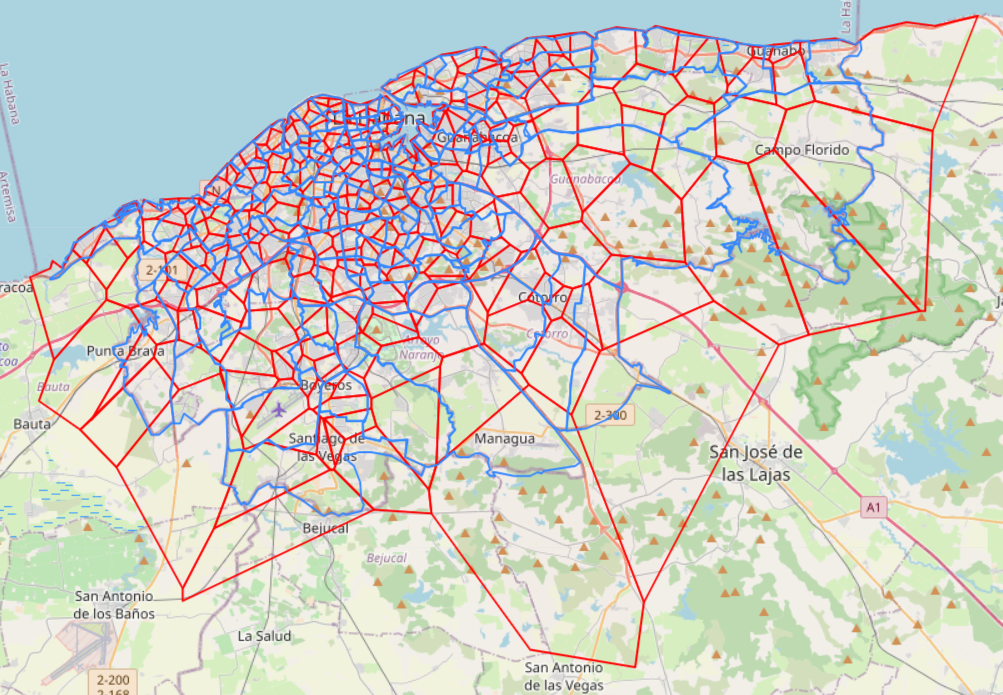
\includegraphics[width=0.9\textwidth]{Graphics/havana_representation.png} \caption{Zonas de transporte de La Habana sobre las zonas de coberturas originadas a partir de los centros de los grupos de torres.} \label{fig:havana_representation} 
\end{figure}

\begin{table}[h!]
\centering
\begin{tabular}{|p{4cm}|p{5cm}|p{5cm}|}
\hline
\textbf{Zonas}        & \textbf{Llegada}               & \textbf{Salida}                \\ \hline
[87, 106, 108, 113]   & [1013, 33742, 34979, 35340]    & [30761, 33742, 34979, 35340]   \\ \hline
[80, 33, 48, 128]     & [29818, 60456, 60527, 61743]   & [60009, 60456, 60527, 61826]   \\ \hline
\end{tabular}
\caption{Secuencias de zonas de transporte y tiempos asociados de entrada y salida a cada zona de transporte en dos viajes.}
\label{tabla:havana_data_format}
\end{table}

Esta metodología de identificación de trayectorias se ha implementado previamente en \cite{garciaborroto2021}, donde se demuestra que las trayectorias extraídas presentan una buena correlación con la información conocida sobre la movilidad en La Habana.

Como cada usuario puede dejar m\'ultiples registros en una misma zona de transporte, se decidi\'o reducir el tama\~no de los datos a partir de identificar exclusivamente la hora en la que se deja la primera se\~nal en una zona (entrada) y la hora en la que se deja la \'ultima (salida), evitando poner todos los registros intermedios. Para cada viaje, se registra la secuencia de zonas de transporte visitadas, así como los tiempos de llegada y salida correspondientes. El tiempo se codifica como un número entero que representa el segundo del día (donde 12:00:01 a.m. corresponde al número 1). De este modo, la información de los viajes se organiza en documentos con líneas formateadas como en la tabla \ref{tabla:havana_data_format}.

\subsection{Caracterización y plausiblidad de los datos}
\label{etecsa_data_description}

Los datos utilizados corresponden al registro del movimiento de usuarios desconocidos durante un período de 54 días consecutivos de actividad normal, comprendido entre el 4 de diciembre de 2021 y el 26 de enero de 2022. La figura \ref{fig:trips_per_day} refleja la dinámica temporal del número de viajes por dia y  se observa claramente una disminución en la actividad cercana a fin de año. Durante este período, la situación del Covid-19 en Cuba era relativamente favorable, lo que sugiere que estos registros de movilidad reflejan un comportamiento representativo y confiable. Inicialmente, se recopilaron un total de 6,456,967 trayectorias a lo largo de los días del estudio. En la figura \ref{fig:trip_duration_histogram} se observa que las trayectorias analizadas presentan una amplia variabilidad en sus duraciones, abarcando desde menos de una hora hasta un día completo. Asimismo, se identificaron paradas que alcanzan incluso las 5 horas de duración. Por esta razón, los datos fueron procesados para garantizar que cumplieran con la definición de viajes establecida en \ref{def:trip}.

\begin{figure}[!htb]
\centering
\begin{minipage}{0.45\textwidth}
    \centering
    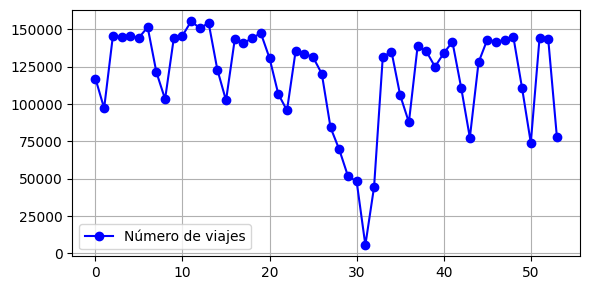
\includegraphics[width=\textwidth]{Graphics/trips_per_day.png}
    \caption{Dinámica temporal del número de viajes por día.}
    \label{fig:trips_per_day}
\end{minipage}%
\hfill
\begin{minipage}{0.45\textwidth}
    \centering
    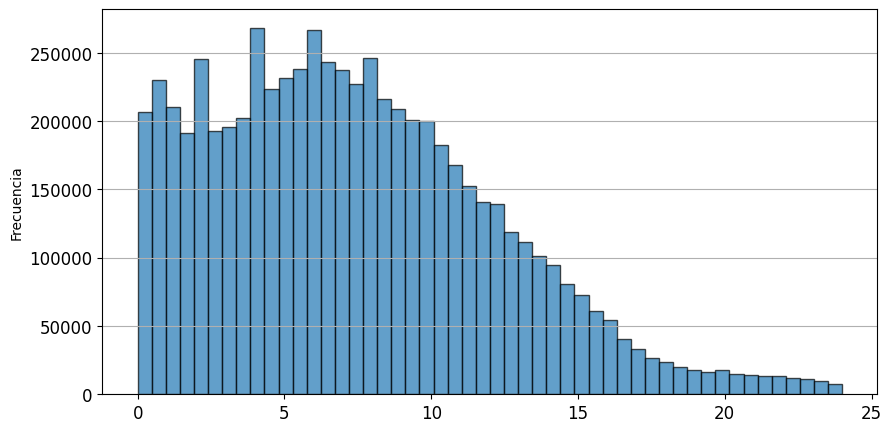
\includegraphics[width=\textwidth]{Graphics/trip_duration_histogram.png}
    \caption{Histograma de frecuencia de las duraciones de los viajes.}
    \label{fig:trip_duration_histogram}
\end{minipage}%
\end{figure}

En la figura \ref{fig:trips_per_timeslot_plot} se observa la distribución de los registros de viajes según la hora de inicio (verde) y la hora de finalización (azul). El gráfico ilustra un comportamiento coherente con los patrones de movilidad urbana: los usuarios tienden a salir en horarios específicos, y sus llegadas suelen ocurrir poco después, reflejando un desplazamiento lógico en el tiempo.

El primer pico de salidas ocurre alrededor de las 6:00 a.m., coincidiendo con el inicio típico de la jornada laboral y escolar. Este pico es seguido de cerca por un incremento en las llegadas, que alcanza su punto máximo alrededor de las 8:00 a.m., lo que sugiere que los desplazamientos durante este horario están vinculados principalmente a traslados hacia centros de trabajo o estudio. Un patrón similar se observa en la tarde: hay un segundo pico importante de salidas entre las 4:00 p.m. y las 5:00 p.m., seguido por un aumento en las llegadas hacia las 6:00 p.m., lo que refleja el regreso a casa al finalizar la jornada.

La clara sincronización entre los horarios de inicio y finalización de los viajes sugiere que los registros reflejan de manera precisa la dinámica diaria de la ciudad. Este patrón proporciona una base sólida para delimitar una ventana de estudio entre las 6:00 a.m. y las 6:00 p.m., ya que dicho intervalo concentra los períodos de mayor actividad y reduce la influencia de registros menos representativos, como los viajes realizados durante horarios nocturnos.

\begin{figure}[!htb] \centering 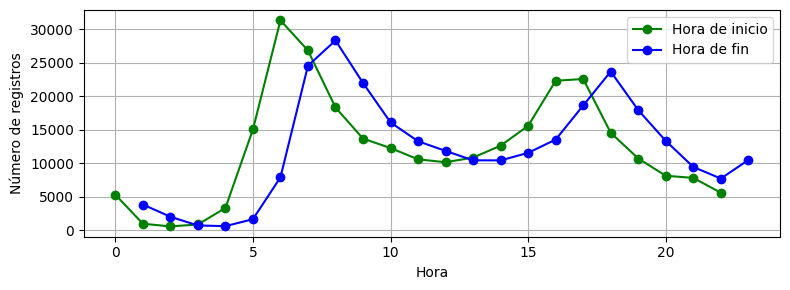
\includegraphics[width=1\textwidth]{Graphics/trips_per_timeslot_plot.png} \caption{Horas de inicio y fin de viajes agregadas en todos los días.} \label{fig:trips_per_timeslot_plot} 
\end{figure}

La figura \ref{fig:register_per_trip_histogram} muestra la distribución de la cantidad de registros por viaje tras filtrar los datos para considerar únicamente los viajes realizados entre las 6:00 a.m. y las 6:00 p.m. Se observa que la mayoría de los viajes tienen entre 4 y 6 registros, mientras que la frecuencia disminuye progresivamente a medida que aumenta el número de registros, lo que indica que los viajes más largos o complejos son menos comunes. Esto resalta que la mayoría de los trayectos son breves en cuanto a la cantidad de puntos registrados, aunque también se incluyen casos de mayor duración. La figura \ref{fig:delta_t_histogram} muestra la distribución de los tiempos entre registros consecutivos en las trayectorias analizadas. La mayoría de los intervalos son cortos, con una mediana de 12.12 minutos y una media ligeramente superior de 18.26 minutos. 

\begin{figure}[!htb]
\centering
\begin{minipage}{0.45\textwidth}
    \centering
    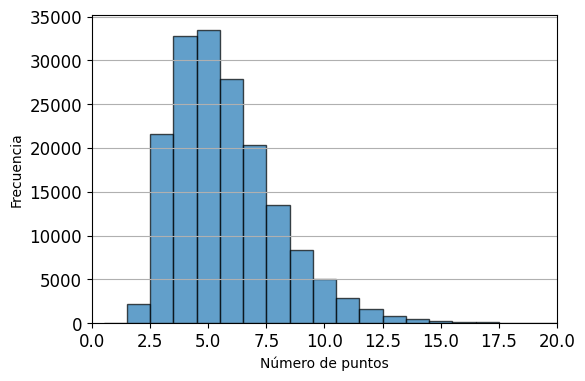
\includegraphics[width=\textwidth]{Graphics/register_per_trip_histogram.png}
    \caption{Histograma de la cantidad de registros por viajes.}
    \label{fig:register_per_trip_histogram}
\end{minipage}%
\hfill
\begin{minipage}{0.45\textwidth}
    \centering
    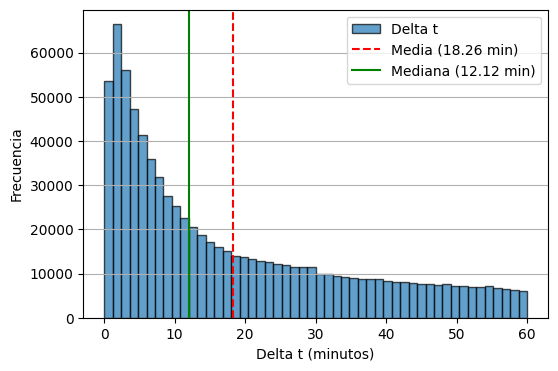
\includegraphics[width=\textwidth]{Graphics/delta_t_histogram.png}
    \caption{Distribución de los intervalos de tiempo ($\Delta t$) entre registros consecutivos.}
    \label{fig:delta_t_histogram}
\end{minipage}%
\end{figure}

Por último, se realizó un análisis de las diferencias en los flujos de transporte entre la mañana y la tarde, evidenciando un patrón de movilidad típico de áreas metropolitanas, como se muestra en la figura \ref{fig:morning_afternoon_difference_coulor}. En la mañana, las zonas periféricas registran un mayor flujo de salidas, representadas por tonos claros, mientras que las zonas centrales, de mayor actividad socioeconómica, muestran un aumento en las llegadas, reflejado en tonos oscuros. Esto evidencia el desplazamiento de personas desde sus hogares hacia zonas de trabajo o servicios. Por el contrario, en la tarde, el flujo se invierte: las personas regresan a sus zonas de residencia en la periferia, mientras que las zonas centrales pierden afluencia. Estos patrones son coherentes con los datos de movilidad previamente observados en La Habana y reportados en \cite{padron2021transporte}.

\begin{figure}[!htb] \centering 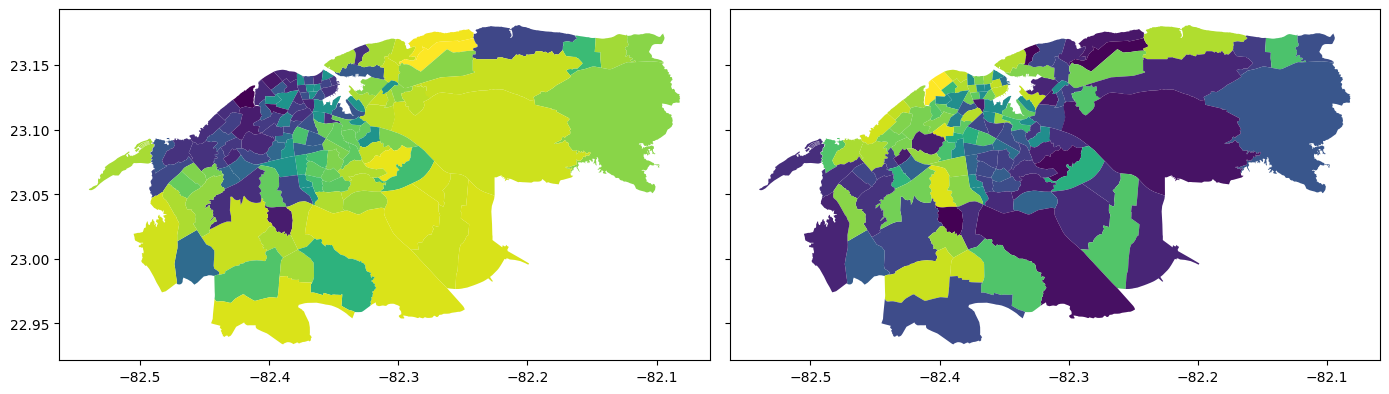
\includegraphics[width=1\textwidth]{Graphics/morning_afternoon_difference_coulor.png} \caption{Diferencia entre salidas y llegadas por zona de transporte: tonos claros indican más salidas, oscuros más llegadas. Izquierda: mañana, derecha: tarde.} \label{fig:morning_afternoon_difference_coulor} 
\end{figure}

En términos generales, los datos son consistentes con investigaciones previas y con el conocimiento que tenemos sobre la ciudad y su dinámica. Esto nos permite asumir que la definición de viajes utilizada es adecuada y captura de manera precisa la movilidad poblacional en La Habana durante el período analizado. En la sección siguiente, aplicamos la metodología propuesta en el capítulo anterior para el completamiento de estas trayectorias.

\section{Experimentación y resultados}

Este experimento tiene como objetivo principal ajustar los hiperparámetros del modelo TrajBERT para optimizar su desempeño sobre los datos de telefonía móvil cubanos. Además, se buscó comparar los resultados obtenidos con un estudio similar realizado recientemente en La Habana, evaluando cómo el modelo podría capturar las relaciones espaciales y temporales específicas de la región.

\begin{figure}[!htb] \centering \includegraphics[width=0.7\textwidth]{Graphics/data_preproccess_flow.pdf} \caption{Ilustraci\'on del proceso de transformaci\'on de los datos en tiempo continuo de los registros LAU al formato requerido por TrajBERT.} \label{fig:data_preproccess_flow} 
\end{figure}

El primer paso fue adaptar el formato de los datos de telefonía móvil cubanos, ver tabla \ref{tabla:havana_data_format}, al formato de entrada de TrajBERT. Para ello, se desarrolló un proceso de transformación que agrupó los datos por viaje, generando trayectorias de longitud fija. Durante este proceso, se asignó a cada intervalo el valor más frecuente de la ubicación registrada como se ilustra en el diagrama 
\ref{fig:data_preproccess_flow}. La distribución observada en \ref{fig:delta_t_histogram} respalda la elección de $\epsilon$, definido en \ref{def:e_sampling}, como 15 minutos, ya que permite capturar la mayoría de los registros frecuentes sin generar redundancia ni perder información relevante sobre las trayectorias. Por lo tanto, para estos datos se tomó $m = 48$, similar a lo hecho en la sección \ref{sec:humob_experiments} y en el trabajo original \cite{si2023trajbert}. 

Los datos fueron particionados con la misma proporción que en la sección \ref{sec:humob_experiments}. El modelo fue entrenado utilizando un equipo de cómputo de alto rendimiento equipado con una tarjeta gráfica NVIDIA GeForce RTX 4090, que cuenta con 24 GB de memoria dedicada y soporte para CUDA 12.7, ofreciendo capacidades excepcionales para cálculos intensivos y entrenamiento de modelos de aprendizaje automático.  

Sobre el conjunto de validación se observó que el rendimiento del modelo mejoraba al incrementar el tamaño del \textit{embedding}, pero comenzaba a decrecer una vez superado un tamaño de 512. Por ello, se seleccionó 512 como el tamaño óptimo para este caso. Además, se identificó que aumentar el número de capas y cabezas de atención disminuía el rendimiento del modelo, lo cual puede atribuirse a que la estructura de las trayectorias son más simples en comparación con datos secuenciales más complejos, como el lenguaje natural. Los patrones de movilidad en la ciudad son periódicos y están limitados por la estructura espacial urbana, lo que implica relaciones estables y simples entre las ubicaciones. Por este motivo, se decidió configurar el modelo con dos capas y dos cabezas de atención, priorizando su capacidad de generalización en este contexto específico. En la figura \ref{fig:etecsa_hiperparameter_variability} se puede observar lo antes mencionado.

\begin{figure}[!htb] \centering 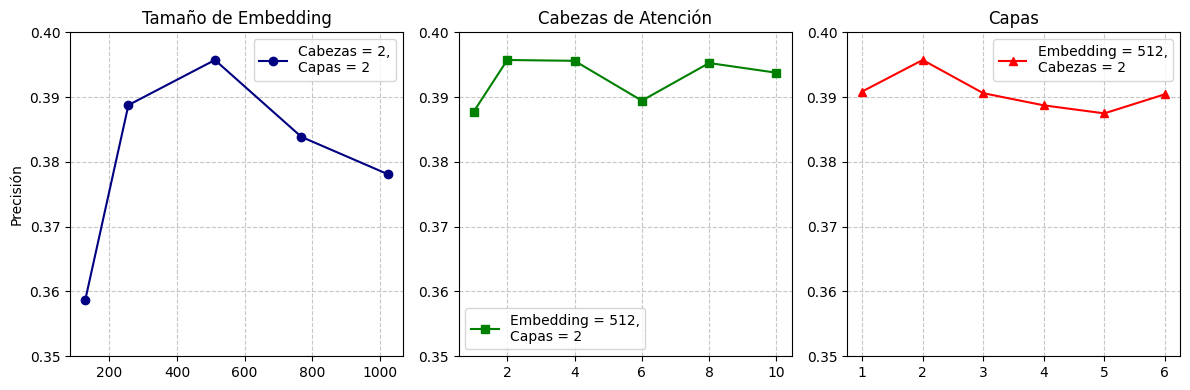
\includegraphics[width=1\textwidth]{Graphics/etecsa_hiperparameter_variability.png} \caption{Relación entre la exactitud y los valores de tamaño del \textit{embedding}, número de cabezas de atención, y número de capas. Los valores de \textit{embedding}, cabezas y capas están fijados en 512, 2 y 2 respectivamente, excepto en la gráfica correspondiente donde se analiza su variación.} \label{fig:etecsa_hiperparameter_variability} 
\end{figure}

El modelo logró una exactitud base de 39.60\% en la clasificación directa sobre el conjunto de prueba, demostrando capacidad inicial de aprendizaje en condiciones reales. Al incorporar métricas de evaluación extendidas, se observa un progreso significativo: la métrica \textit{fuzzy-acc} alcanza 57.19\%, mientras que los resultados en \textit{top-3}, \textit{top-5} y \textit{top-10} muestran valores de 58.87\%, 62.83\% y 68.51\% respectivamente, lo que indica una tendencia positiva en la identificación de patrones espaciales. En cuanto a la precisión geográfica, la distancia promedio entre predicciones y valores reales fue de 3.82 km, un resultado inicial que establece un punto de referencia para optimizaciones futuras.

Para evaluar el impacto de la completitud de los datos en el modelo, se introdujo el concepto de densidad de trayectorias, definido como la proporción de puntos conocidos respecto a la longitud total de la secuencia (excluyendo los tokens de \textit{padding} en los extremos). El análisis de la densidad de trayectorias reveló patrones clave sobre la adaptabilidad del modelo.

Las trayectorias del conjunto de prueba se clasificaron en tres niveles: baja (<50\% de datos conocidos), media (50\%-80\%) y alta (>80\%). Como se observa en la figura \ref{fig:accuracy_metrics}, existe una correlación positiva entre completitud y desempeño: la exactitud aumentó de 36.60\% en trayectorias de baja densidad a 44.43\% en aquellas de alta densidad. Además, las métricas extendidas mostraron una mayor resiliencia, con un \textit{top-10} que alcanzó el 78.20\% en trayectorias de alta densidad y se mantuvo en 61.68\% incluso en secuencias con baja densidad. Complementando este análisis, la figura \ref{fig:geospatial_distance} muestra que la distancia geoespacial promedio disminuyó progresivamente con el aumento de la densidad, evidenciando que las trayectorias más completas permiten una localización más precisa.

\begin{figure}[!htb]
\centering
\begin{minipage}{0.45\textwidth}
    \centering
    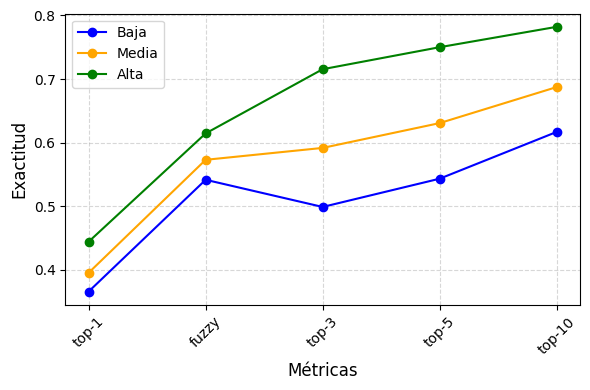
\includegraphics[width=\textwidth]{Graphics/accuracy_metrics.png}
    \caption{Comportamiento de las métricas de exactitud al variar las densidades.}
    \label{fig:accuracy_metrics}
\end{minipage}%
\hfill
\begin{minipage}{0.45\textwidth}
    \centering
    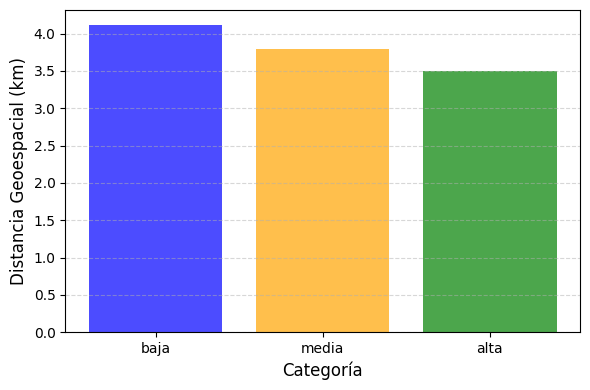
\includegraphics[width=\textwidth]{Graphics/geospatial_distance.png}
    \caption{Comportamiento de la distancia geoespacial promedio al variar las densidades.}
    \label{fig:geospatial_distance}
\end{minipage}%
\end{figure}

Los resultados muestran que, si bien la densidad de datos afecta el desempeño del modelo, este sigue siendo capaz de sugerir ubicaciones geográficas plausibles, evidenciando su potencial en análisis de movilidad a gran escala. No obstante, al procesar puntos de forma aislada en contextos de alta incertidumbre se pierden las dependencias espaciotemporales, lo que incrementa los errores y reduce la efectividad. Esto valida que la integración del contexto secuencial optimiza el manejo de datos fragmentados.

Para dar sentido relativo a estos resultados, en el siguiente ep\'igrafe se comparan con los obtenidos usando otro esquema m\'as simple de redes neuronales.

\section{Completamiento de trayectorias con ANN}

En la revisión bibliográfica, se identificaron varios estudios \cite{rodriguez2022movilidad, padron2021transporte, garciaborroto2021, durive2021sistema} que abordan el uso de datos de telefonía móvil para identificar patrones de movilidad en Cuba. En particular, uno de ellos propone un modelo basado en redes neuronales artificiales para la \textit{Reconstrucción de Trayectorias en Puntos Intermedios} (IPPR, por sus siglas en inglés) \cite{rodriguez2022movilidad}. Este modelo predice la ubicación intermedia de un viajero a partir de su origen, destino y una fracción del trayecto completada.

El modelo recibe como entrada cinco valores: la latitud y longitud del punto de origen, la latitud y longitud del destino, y un valor en el intervalo $[0,1]$ que representa el progreso del viaje. La salida es una distribución de probabilidad sobre 134 zonas de transporte, obtenida mediante una capa \textit{softmax}. La red neuronal emplea una arquitectura de tres capas ocultas totalmente conectadas, ver figura \ref{fig:ann_architecture}. El entrenamiento del modelo se realizó utilizando el optimizador Adam, minimizando la divergencia de Kullback-Leibler \cite{van2014renyi}.

\begin{figure}[!htb]
\centering
\begin{minipage}{0.50\textwidth}
    \centering
    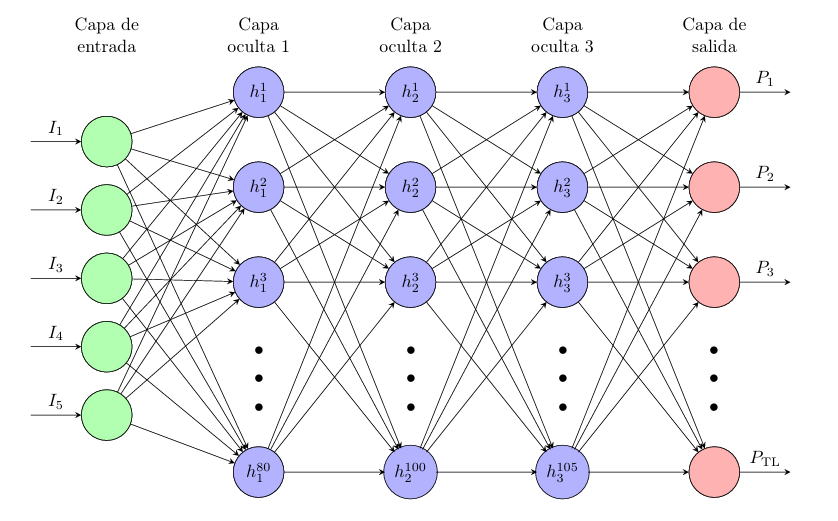
\includegraphics[width=\textwidth]{Graphics/ann_architecture.png}
    \caption{Arquitectura de la ANN para la \textit{Reconstrucción de Trayectorias en Puntos Intermedios}, figura extraída de \cite{rodriguez2022movilidad}.}
    \label{fig:ann_architecture}
\end{minipage}%
\hfill
\begin{minipage}{0.45\textwidth}
    \centering
    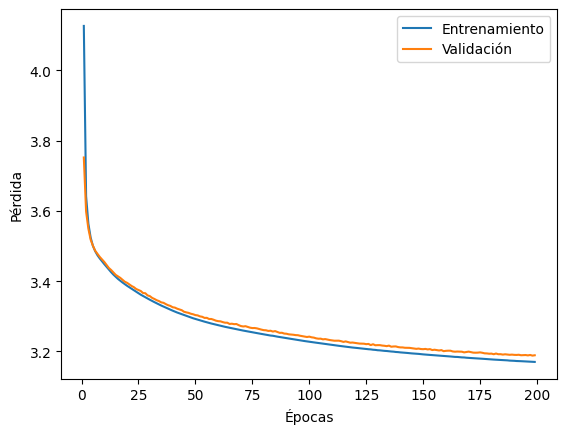
\includegraphics[width=\textwidth]{Graphics/ann_loss.png}
    \caption{Comportamiento de la función de pérdida en los conjuntos de entrenamiento y validación.}
    \label{fig:ann_loss}
\end{minipage}%
\end{figure}

Establecer una comparación directa entre TrajBERT y los resultados expuestos en \cite{rodriguez2022movilidad} resulta muy difícil, ya que, aunque ambos modelos fueron entrenados con el mismo conjunto global de datos, el filtrado y la segmentación aplicados fueron diferentes. En \cite{rodriguez2022movilidad} se trabajó únicamente con registros tomados de 6:00 a.m. a 10:00 a.m., y se presentan resultados luego de dividir el conjunto de prueba en tres subconjuntos en función de la distancia entre los \textit{ID de ubicación} de origen y destino de cada trayectoria. Esta estrategia difiere evidentemente de la empleada en este trabajo, lo que imposibilita una comparación directa de los desempeños reportados.

Por lo tanto, con el fin de comparar el modelo propuesto en \cite{rodriguez2022movilidad} con los resultados de TraBERT, se optó por reentrenar la ANN utilizando las mismas especificaciones propuestas, pero esta vez con los datos descritos en la sección \ref{etecsa_data_description}. El objetivo era partir de la misma base de conocimiento para ambos modelos, permitiendo así una comparación justa en términos de capacidad de generalización y desempeño. En la figura \ref{fig:ann_loss} se muestra el comportamiento de la función de pérdida en los conjuntos de entrenamiento y validación durante 200 épocas, mostrando cómo el modelo converge consistentemente.

\subsection{Comparación con TrajBERT}

Aunque el modelo propuesto en \cite{rodriguez2022movilidad} resulta ingenioso, presenta una limitación crítica: no aprovecha de manera adecuada la información contextual inherente a las trayectorias secuenciales. Las trayectorias urbanas no son simplemente colecciones de puntos aislados, sino secuencias espaciotemporales en las que la elección de una zona de transporte depende de decisiones previas y de patrones de movilidad subyacentes. La arquitectura de la ANN, al procesar cada cuadrupleta (origen, intermedio, destino, fracción de tiempo) de forma independiente, ignora las dependencias a largo plazo y la estructura secuencial que modelos como TrajBERT capturan mediante mecanismos de atención.

Los resultados numéricos de la tabla \ref{tab:etecsa_model_comparison} reflejan esta brecha. Mientras la ANN alcanza una exactitud del 18.92\% y una distancia geográfica promedio de 4.82 km, TrajBERT duplica la exactitud (39.60\%) y reduce el error geográfico a 3.82 km. Además, en métricas que evalúan la flexibilidad de las predicciones (\textit{top-3}, \textit{top-5} y \textit{top-10}), TrajBERT supera consistentemente a la ANN, lo que sugiere una mayor capacidad para generar distribuciones de probabilidad mejor calibradas y contextualmente relevantes.

\begin{table}[ht]
\centering
\begin{tabular}{|l|c|c|c|c|c|}
\hline
\textbf{Modelo} & \textbf{Exactitud} & \textbf{top-3} & \textbf{top-5} & \textbf{top-10} & \textbf{Distancia (km)} \\ \hline
ANN             & 0.1892                & 0.3924            & 0.5122            &  0.6786            & 4.8170                  \\ \hline
TrajBert        & 0.3960                & 0.5887            & 0.6283            & 0.6851             & 3.8238                  \\ \hline
\end{tabular}
\captionof{table}{Comparación de resultados entre la ANN y TrajBERT.}
\label{tab:etecsa_model_comparison}
\end{table}

Los resultados indican que, al basarse únicamente en puntos intermedios, la ANN no logra capturar de forma efectiva la compleja estructura espacial de La Habana. En cambio, TrajBERT, gracias a su refinamiento espaciotemporal (sección \ref{trajectory_encoder}) y la función STAL (sección \ref{stal_function}), extrae patrones geográficos con mayor precisión, lo que se refleja en un desempeño superior en el completamiento de trayectorias.

Evaluar el impacto de la densidad de trayectorias en la ANN no tiene fundamentación metodológica, ya que este modelo no procesa la información en forma secuencial. Por lo tanto, las variaciones en la densidad no influyen en la comprensión de una trayectoria en particular. Sin embargo, siguiendo el enfoque de \cite{rodriguez2022movilidad}, que define la distancia origen-destino como el número mínimo de aristas entre nodos en el grafo de zonas de transporte de La Habana, nuestro análisis (ver figura \ref{fig:distance_variability}) revela que ambos modelos mantienen una estabilidad métrica frente a trayectorias de distancias crecientes, con TrajBERT mostrando un rendimiento superior. Este resultado contrasta con lo reportado en \cite{rodriguez2022movilidad}, donde se observa una degradación en la efectividad del completamiento de trayectorias más largas. Las trayectorias se clasificaron en tres niveles: corta (<6 aristas entre los nodos origen-destino), media (6-8) y lejana (>8).

\begin{figure}[!htb] \centering 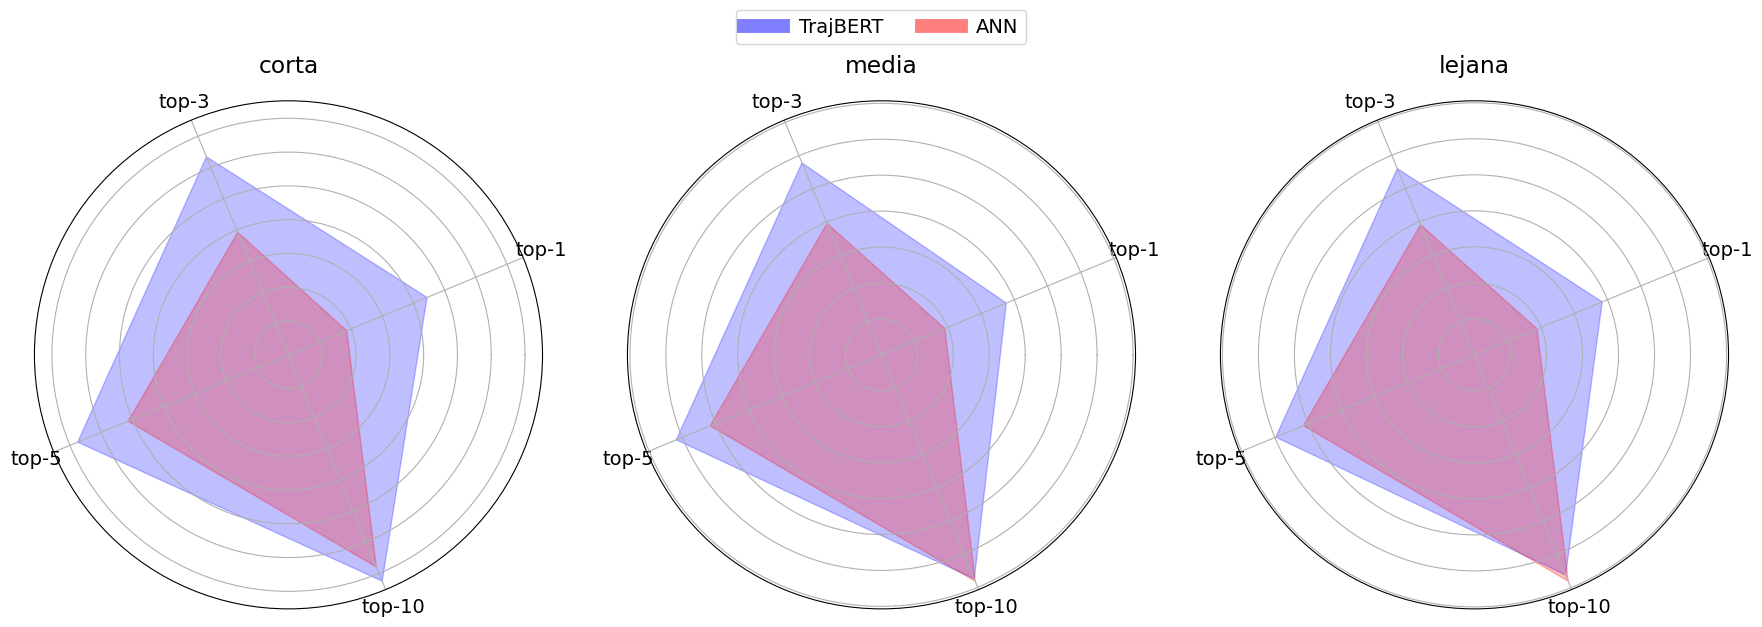
\includegraphics[width=1\textwidth]{Graphics/distance_variability.png} \caption{Comparación de las métricas de exactitud entre TrajBERT y la ANN de \cite{rodriguez2022movilidad} al variar la distancia entre los \textit{ID de ubicación} de origen y destino.} \label{fig:distance_variability} 
\end{figure}

La discrepancia en el comportamiento de la ANN puede explicarse por diferencias en la calidad o distribución de los datos y las condiciones de entrenamiento. Por lo tanto, se concluye que, al menos en este conjunto de datos, TrajBERT ofrece un desempeño significativamente superior.

\backmatter

\begin{conclusions}

    Los resultados presentados en este trabajo permiten afirmar que se han cumplido los objetivos específicos y se ha corroborado la hipótesis de trabajo formulada en la introducción. Efectivamente, el uso de un modelo de aprendizaje automático basado en \textit{transformers} permite capturar las complejas relaciones espaciotemporales que existen entre las ubicaciones de una trayectoria.
    
    La aplicación de TrajBERT para el completamiento de trayectorias implícitas a partir de datos de telefonía móvil en Cuba demuestra la viabilidad de un enfoque avanzado en un entorno con datos bastante dispersos. Se evidenció que su innovadora arquitectura, que incorpora un refinamiento espaciotemporal y la función STAL, realmente ofrece mejoras significativas en el rendimiento del modelo, superando los números alcanzados por el enfoque previo cubano con una arquitectura más simple basado en redes neuronales artificiales.
    
    Al comparar los experimentos realizados con los conjuntos de datos de ETECSA y \textit{HuMob}, se observa que en el contexto cubano el rendimiento del modelo es inferior, lo que apunta a una limitación atribuible a la calidad del conjunto de datos y no al método en sí. Esto sugiere que, si se contara con datos de entrenamiento de mayor precisión y densidad, por ejemplo, obtenidos mediante dispositivos GPS, el modelo podría alcanzar niveles de eficiencia en Cuba aún mayores, incluso en escenarios con datos muy dispersos.
    
    Los alcances prácticos de esta investigación son evidentes. Las aplicaciones potenciales van desde la modelación de la propagación de enfermedades basada en patrones de movilidad inferidos hasta la selección óptima de ubicaciones para la construcción de tiendas u hospitales. Otra propuesta interesante es la compresión y descompresión de datos de movilidad, es decir, representar trayectorias completas mediante un subconjunto crítico de puntos, lo que reduciría el volumen de almacenamiento requerido sin perder la utilidad analítica. En este sentido, TrajBERT podría desempeñar un papel clave al ``descomprimir'' estos datos, permitiendo obtener de vuelta la información detallada a partir de representaciones comprimidas.
    
    El análisis desarrollado en este trabajo, junto con la difusión de la base de código a la comunidad científica cubana, abre nuevas líneas de investigación para optimizar la aplicación de técnicas de aprendizaje profundo en el estudio de la movilidad humana en Cuba. Estos avances permitirán una comprensión más precisa de los patrones de movilidad y favorecerán el diseño de estrategias innovadoras en ámbitos tan relevantes como la planificación urbana, el transporte, los estudios epidemiológicos y la toma de decisiones en políticas públicas.
        
\end{conclusions}
\begin{recomendations}
    Recomendaciones
\end{recomendations}

\printbibliography[heading=bibintoc]


\end{document}